% =====================================================================
%  DSP391m · Group 5 — Task 3: Data Collection & Preprocessing (English)
%  Beamer deck styled to match reports/guide/DataTask_Process_Guide.pdf
%  (maroon #800000 + cream, Latin Modern serif, booktabs, takeaways).
%  Compile with Tectonic (XeTeX):  tectonic Task3_Slides_EN.tex
% =====================================================================
\documentclass[aspectratio=169,11pt]{beamer}

\usetheme{default}
\setbeamertemplate{navigation symbols}{}
\usefonttheme{serif}                 % Latin Modern serif, like the guide

\usepackage{iftex}
\ifPDFTeX
  \usepackage[T1]{fontenc}
  \usepackage[utf8]{inputenc}
  \usepackage{lmodern}
\else
  \usepackage{fontspec}              % XeTeX/Tectonic: real Latin Modern OTF
\fi
\usepackage{booktabs}
\usepackage{array}
\usepackage{tabularx}
\usepackage{colortbl}
\usepackage{graphicx}
\graphicspath{{../figures/}{figures/}{./}}

% ---- colours (identical to the guide) ----
\definecolor{themecol}{HTML}{800000}   % maroon
\definecolor{rowtint}{HTML}{F3E9E9}    % cream
\definecolor{codebg}{HTML}{F6F4F0}
\definecolor{cgreen}{HTML}{2E7D32}
\definecolor{cblue}{HTML}{1F5C99}
\definecolor{cgrey}{HTML}{6B6B6B}

\setbeamercolor{structure}{fg=themecol}
\setbeamercolor{frametitle}{fg=themecol}
\setbeamercolor{title}{fg=themecol}
\setbeamercolor{itemize item}{fg=themecol}
\setbeamercolor{itemize subitem}{fg=cgrey}
\setbeamerfont{frametitle}{series=\bfseries}
\setbeamertemplate{itemize item}{\textbullet}
\setbeamertemplate{itemize subitem}{\textendash}

% ---- thin maroon footline like the guide's header/footer ----
\setbeamertemplate{footline}{%
  \hbox{\begin{beamercolorbox}[wd=\paperwidth,ht=2.6ex,dp=1.2ex,leftskip=1.2em,rightskip=1.2em]{}%
    {\color{cgrey}\scriptsize DSP391m · Group 5 · Task 3 — Data Collection \& Preprocessing}%
    \hfill{\color{cgrey}\scriptsize\insertframenumber}%
  \end{beamercolorbox}}%
}

% ---- helpers (match the guide) ----
\newcolumntype{Y}{>{\raggedright\arraybackslash}X}
\newcommand{\hc}[1]{{\bfseries\color{white}#1}}
\newcommand{\code}[1]{\texttt{\detokenize{#1}}}
\newcommand{\takeaway}[1]{\vspace{2pt}\par{\footnotesize\itshape\textcolor{themecol}{$\Rightarrow$\,}#1}}
\newcommand{\keynum}[1]{\vspace{2pt}\par{\small\textcolor{themecol}{$\blacktriangleright$ \textbf{Key:}}\ #1}}
% What / Why / Result bullets (the deck's signature structure, in guide colours)
\newcommand{\wwr}[3]{%
  \begin{itemize}\setlength\itemsep{0.45em}
    \item[\textcolor{cgreen}{\textbf{What}}]\,#1
    \item[\textcolor{cblue}{\textbf{Why}}]\,#2
    \item[\textcolor{themecol}{\textbf{Result}}]\,#3
  \end{itemize}}
% maroon part-divider frame
\newcommand{\partframe}[3]{%
  {\setbeamercolor{background canvas}{bg=themecol}%
  \begin{frame}[plain]
    \vfill\hspace{1.2em}\begin{minipage}{0.9\textwidth}
      {\color{white!85}\large\textbf{PART #1}}\\[4pt]
      {\color{white}\rule{3.2cm}{2.4pt}}\\[10pt]
      {\color{white}\huge\textbf{#2}}\\[12pt]
      {\color{white!80}\itshape Presenter: #3}
    \end{minipage}\vfill
  \end{frame}}}

\setbeamertemplate{section in toc}{\inserttocsectionnumber.~\inserttocsection}

% ---------------------------------------------------------------- meta
\title{\textbf{Data Collection \& Preprocessing}}
\subtitle{EduGuard: AI-Powered Early Warning and Actionable Recourse System --- Task 3}
\author{Group 5 --- DSP391m}
\institute{FPT University \textbullet{} Supervisor: Phan Duy Hung}
\date{Members: Vinh Le \textbullet{} Ngoc Sang \textbullet{} Van Son \textbullet{} Huy Anh}

\begin{document}

% ===================================================================== Title
{\setbeamercolor{background canvas}{bg=themecol}
\begin{frame}[plain]
  \vfill\hspace{1.1em}\begin{minipage}{0.92\textwidth}
    {\color{white!85}\large\textbf{DATA TASK REPORT}}\\[6pt]
    {\color{white}\rule{3.2cm}{2.4pt}}\\[10pt]
    {\color{white}\huge\textbf{Data Collection \& Preprocessing}}\\[10pt]
    {\color{white!90}\large\itshape EduGuard: AI-Powered Early Warning \& Actionable Recourse System --- Task 3}\\[16pt]
    {\color{white!80}\small DSP391m · Data Science Capstone · Group 5 · FPT University\\
     Supervisor: Phan Duy Hung \quad\textbullet\quad Members: Vinh Le · Ngoc Sang · Van Son · Huy Anh}
  \end{minipage}\vfill
\end{frame}}

% ===================================================================== Agenda
\begin{frame}{Agenda}
  \begin{itemize}\setlength\itemsep{0.5em}
    \item \textbf{Part 1} — Defining the required data \hfill(Son)
    \item \textbf{Part 2} — Data collection method \hfill(Phuc)
    \item \textbf{Part 3} — Data cleaning \hfill(Huy Anh)
    \item \textbf{EDA block} — Exploratory data analysis \hfill(Duc)
    \item \textbf{Part 4} — Transformation \& standardisation \hfill(Binh)
    \item \textbf{Part 5} — Train/test split \& leakage control \hfill(Văn Vinh)
  \end{itemize}
  \takeaway{Every item follows the same frame: \textit{What — Why — Result}.}
\end{frame}

% ===================================================================== Big picture
\begin{frame}{The Big Picture — Our Data Pipeline}
  \begin{columns}[T]
    \begin{column}{0.52\textwidth}
      \wwr{7 raw OULAD tables $\to$ merge $\to$ \code{master_raw} (32{,}593 $\times$ 33) $\to$ cut at 6 time checkpoints $\to$ leakage-safe preprocessing $\to$ train/test.}
          {Huy Anh ``anchor'' slide so we always know which pipeline step we are in.}
          {6 datasets \code{dataset_t10}\ldots\code{t100} + a fixed 20\% test set; \textbf{19/19} leakage tests pass.}
    \end{column}
    \begin{column}{0.48\textwidth}
      \centering
      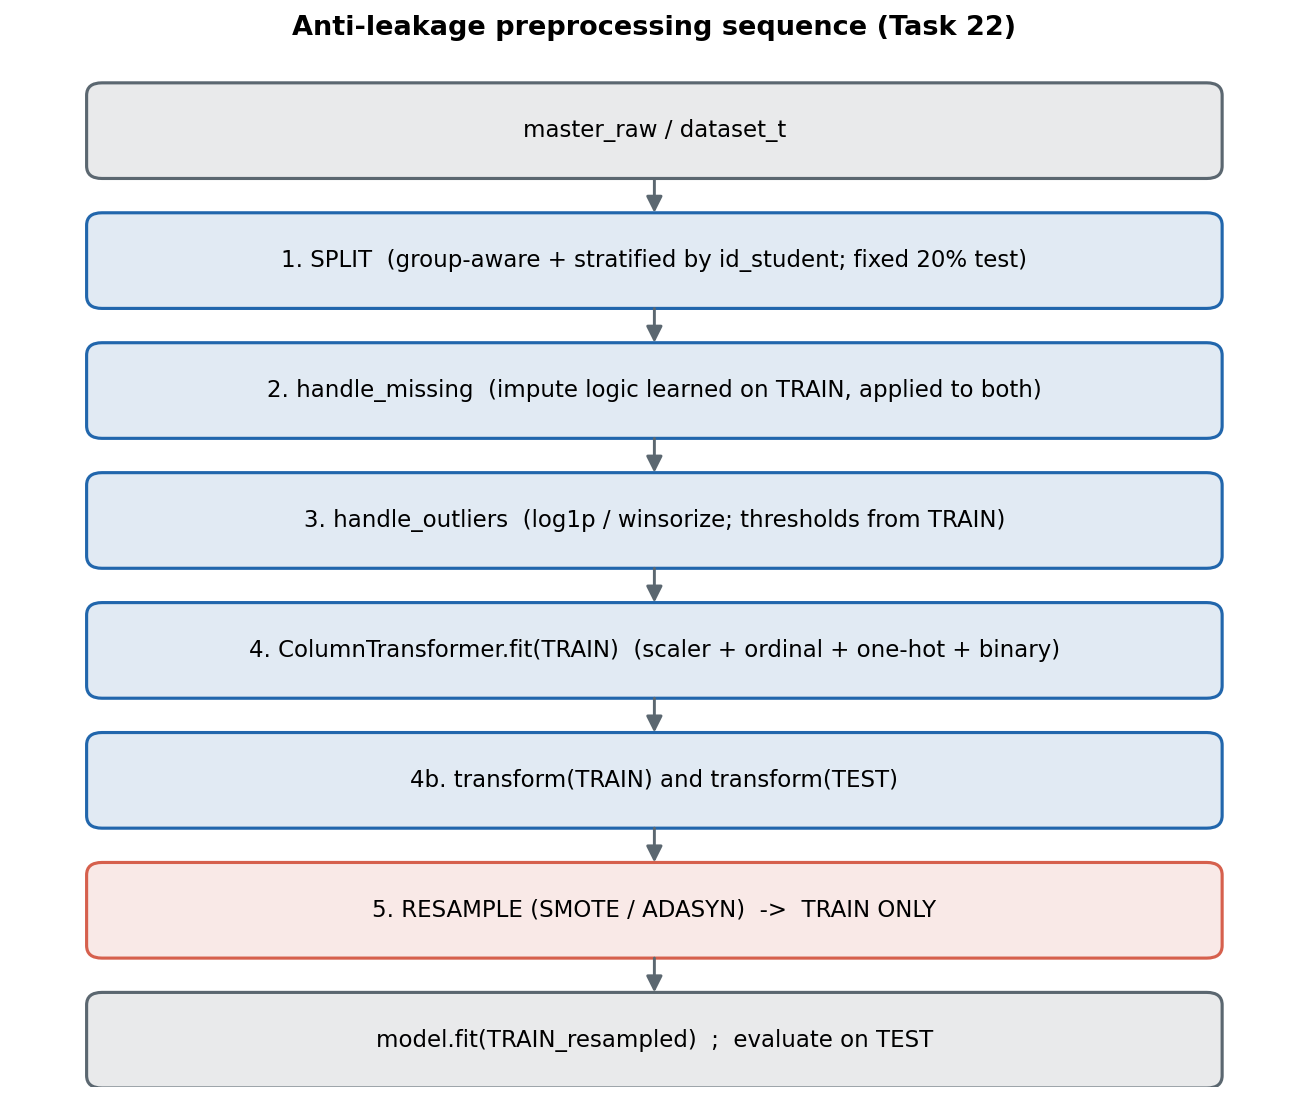
\includegraphics[width=\linewidth,height=0.72\textheight,keepaspectratio]{preprocessing_sequence.png}\\
      {\scriptsize\itshape Anti-leakage preprocessing sequence}
    \end{column}
  \end{columns}
\end{frame}

% ===================================================================== PART 1
\partframe{1}{Defining the Required Data}{Son}

\begin{frame}{Problem \& Objective}
  \wwr{Detect \textbf{early} the students at risk of poor performance on the VLE, and \textbf{explain} every prediction.}
      {Three gaps in prior work: model opacity, late prediction, and class imbalance.}
      {The data must serve RQ1 (early prediction), RQ2 (explanation stability), RQ3 (imbalance).}
\end{frame}

\begin{frame}{Target Variable (\code{at_risk})}
  \begin{columns}[T]
    \begin{column}{0.54\textwidth}
      \wwr{Binary classification: \code{at_risk} derived from \code{final_result}; at-risk (1) = Fail + Withdrawn, not-at-risk (0) = Pass + Distinction.}
          {Group by ``does this student need intervention'' — exactly the early-warning goal.}
          {Real distribution, not 68/32.}
      \keynum{at-risk \textbf{52.8\%} (17{,}208) vs not-at-risk \textbf{47.2\%} (15{,}385).}
    \end{column}
    \begin{column}{0.46\textwidth}
      \centering
      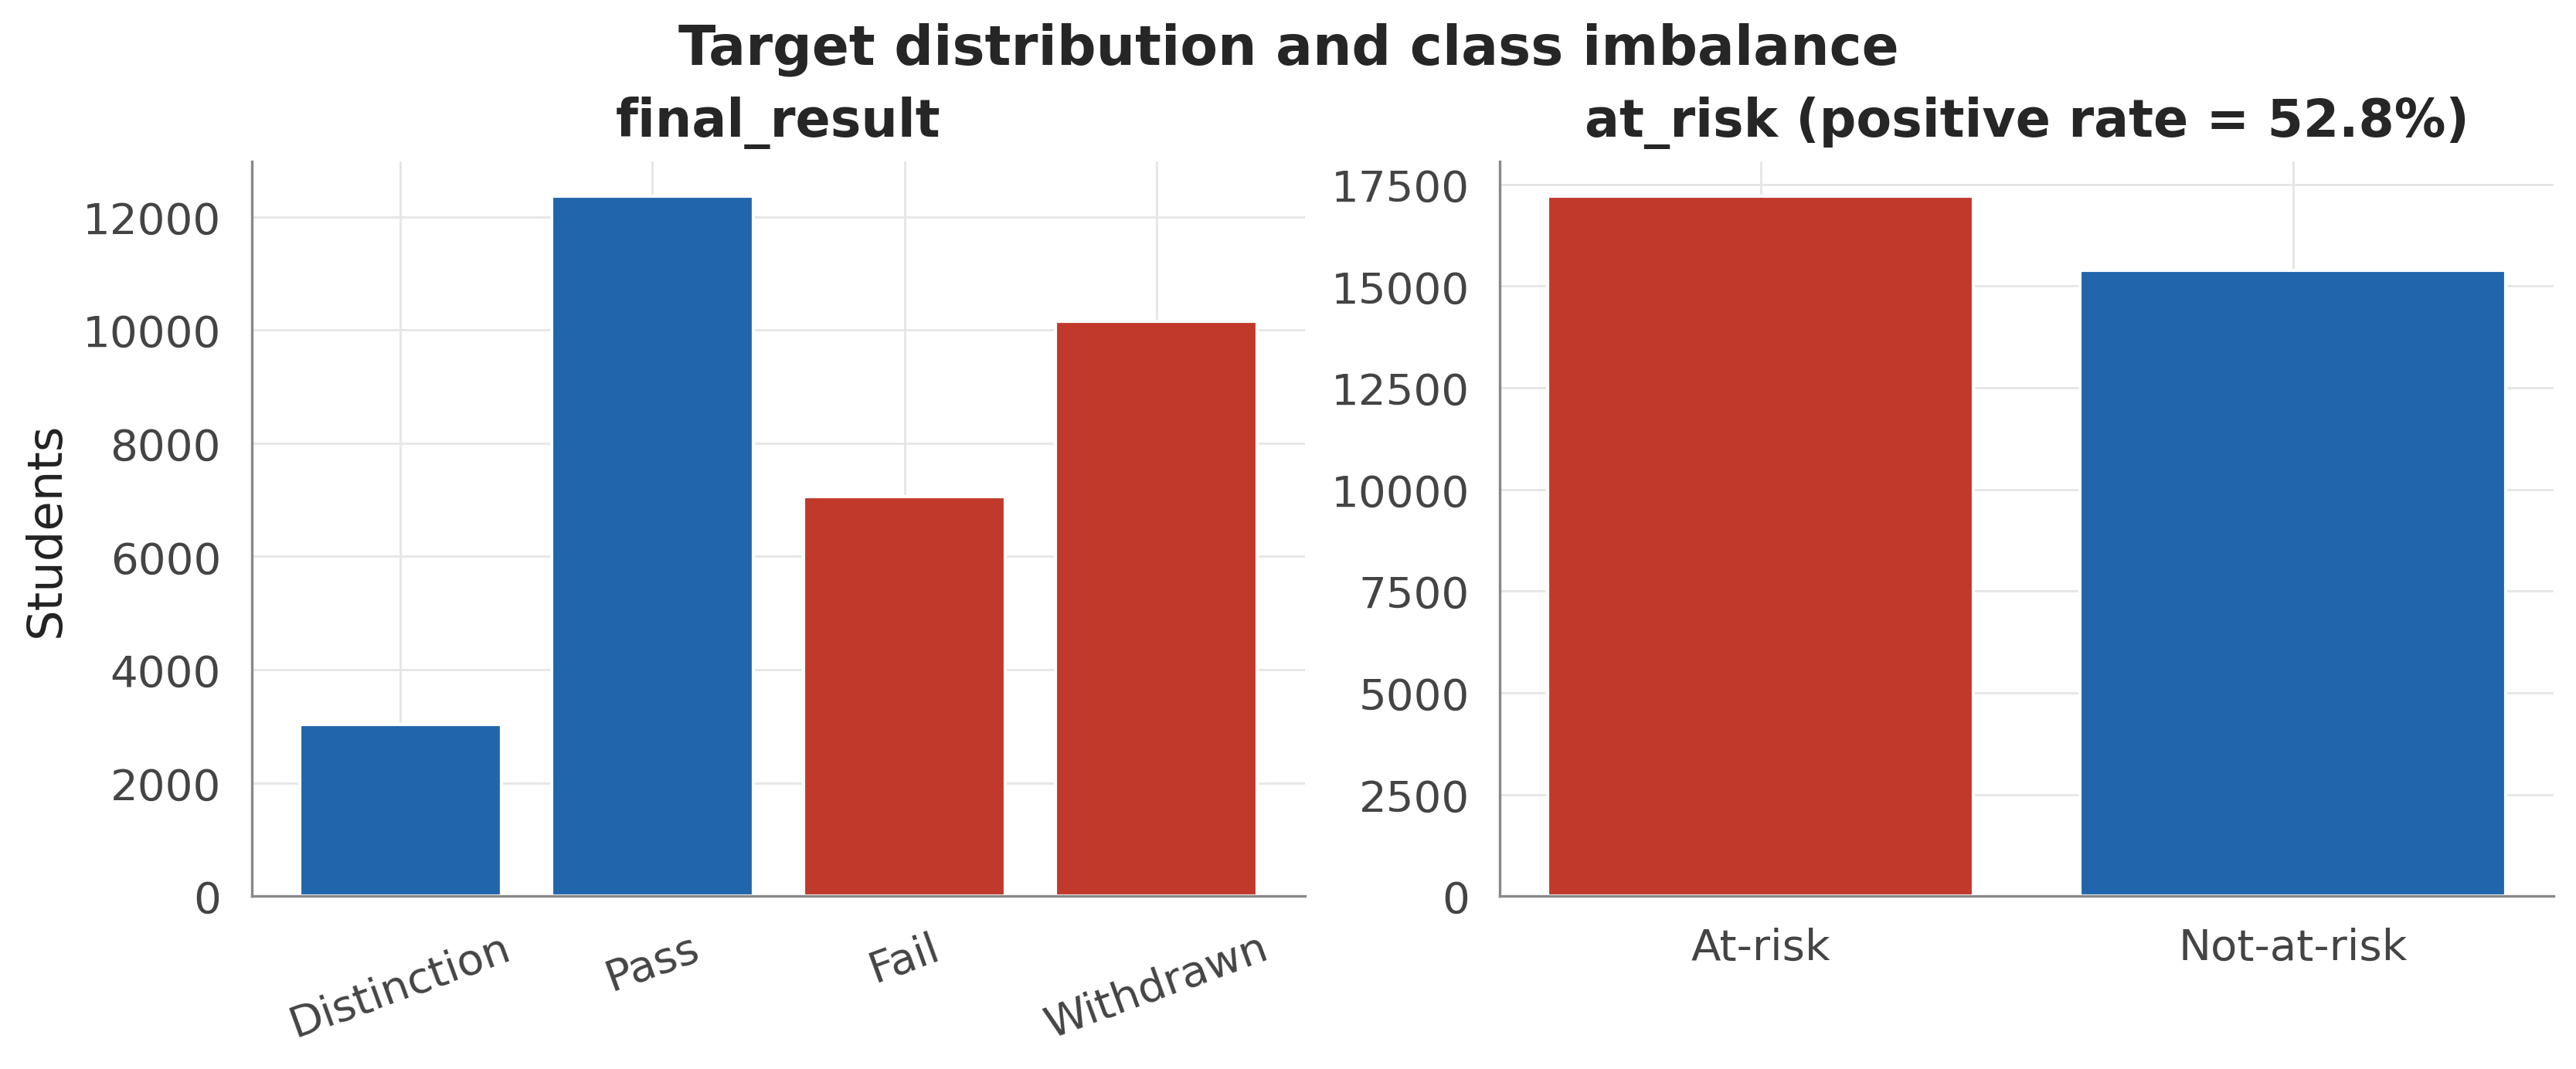
\includegraphics[width=\linewidth,height=0.7\textheight,keepaspectratio]{target_distribution.png}\\
      {\scriptsize\itshape Target distribution \& class imbalance}
    \end{column}
  \end{columns}
\end{frame}

\begin{frame}{Three Input Feature Groups}
  \wwr{Three feature groups: \textbf{Demographic} (gender, region, education, imd\_band, age\_band, disability); \textbf{Engagement/VLE} (clickstream: total/typed clicks, active days); \textbf{Assessment} (submission scores, count, not-submitted flag).}
      {Demographics = context \& fairness; engagement = early behavioural signal; assessment = evidence of performance.}
      {A feature set split into 3 clear groups $\Rightarrow$ group-wise SHAP/LIME interpretation.}
\end{frame}

\begin{frame}{Observation Unit, Scope \& Exclusions}
  \begin{itemize}\setlength\itemsep{0.4em}
    \item[\textcolor{cgreen}{\textbf{Unit}}]\, One row = one student–module–presentation \big(\code{code_module} $\times$ \code{code_presentation} $\times$ \code{id_student}\big).
    \item[\textcolor{cgreen}{\textbf{Scope}}]\, 32{,}593 records · 22 module-presentations · 7 tables · Open University 2013–2014.
    \item[\textcolor{cgreen}{\textbf{Exclude}}]\, Drop identifiers; \textbf{never} use \code{date_unregistration} as a feature; drop the raw \code{final_result}.
    \item[\textcolor{cblue}{\textbf{Why}}]\, Fixing the unit and excluding leaky columns early prevents leakage and row duplication.
  \end{itemize}
\end{frame}

% ===================================================================== PART 2
\partframe{2}{Data Collection Method}{Phuc}

\begin{frame}{Source \& Data Type}
  \wwr{Source: Open University Learning Analytics Dataset (OULAD), Kuzilek et al.\ (2017); type: public \textbf{secondary} data, anonymised at source, CC-BY 4.0.}
      {Ethics satisfied by correct citation; no sensitive personal data is processed.}
      {Legal, reproducible, no primary collection needed — fits an academic setting.}
\end{frame}

\begin{frame}{Collection \& the 7 Tables}
  \wwr{Download 7 CSVs $\to$ \code{data/raw/} $\to$ verify integrity with MD5 (\code{data_manifest.txt}). Tables: studentInfo, courses, studentRegistration, studentVle (\textbf{10{,}655{,}280} rows), vle, assessments, studentAssessment.}
      {Separate light base tables from the heavy clickstream $\to$ chunked processing (500k rows) avoids memory blow-up.}
      {Raw data ``frozen'' + checksummed $\Rightarrow$ everyone uses exactly one version.}
\end{frame}

\begin{frame}{Relationships Between Tables}
  \begin{itemize}\setlength\itemsep{0.4em}
    \item[\textcolor{cgreen}{\textbf{What}}]\, Primary keys:
      \begin{itemize}\setlength\itemsep{0.15em}
        \item \code{(code_module, code_presentation, id_student)} — studentInfo $\leftrightarrow$ registration $\leftrightarrow$ VLE-agg $\leftrightarrow$ performance.
        \item \code{id_site} — studentVle $\leftrightarrow$ vle (activity type).
        \item \code{id_assessment} — studentAssessment $\leftrightarrow$ assessments (weight/deadline).
      \end{itemize}
    \item[\textcolor{cblue}{\textbf{Why}}]\, Knowing the keys is the precondition to merge \textbf{without duplication} (\code{validate='many_to_one'}).
    \item[\textcolor{themecol}{\textbf{Result}}]\, A relational schema — the basis for the Part-3 merge.
  \end{itemize}
\end{frame}

\begin{frame}{Source Evaluation: Fit · Pros · Limits · Risks}
  \wwr{Fit: all 3 feature groups + timestamps $\to$ enables time-aware prediction; 32k is large enough. Pros: international benchmark, anonymised, reproducible, free.}
      {Limits: secondary, single institution; clicks are counts only (no content); 2013–2014 cohorts.}
      {Risks: mild imbalance · structural missingness · strong right-skew · multicollinearity · temporal leakage — all addressed in Parts 3–5.}
\end{frame}

% ===================================================================== PART 3
\partframe{3}{Data Cleaning}{Huy Anh}

\begin{frame}{Raw-Data Overview}
  \wwr{After merging: 32{,}593 rows $\times$ 33 columns; audit data types \& structure.}
      {A ``general check-up'' before intervening — know the scale and variable kinds.}
      {A rows–columns–type summary as the baseline for cleaning.}
\end{frame}

\begin{frame}{Missing Data — Detection \& Strategy}
  \begin{columns}[T]
    \begin{column}{0.52\textwidth}
      \wwr{Only 3 columns missing; missing scores = ``not submitted yet'' $\to$ fill 0 + \code{not_submitted} flag.}
          {Each mechanism (MCAR/MAR/MNAR) is handled differently; ``not submitted'' is \textbf{signal}, not noise.}
          {After handling: \textbf{0} missing in every feature column.}
      {\scriptsize
      \setlength{\tabcolsep}{4pt}\renewcommand{\arraystretch}{1.25}
      \begin{tabularx}{\linewidth}{@{}>{\ttfamily}l r Y@{}}
        \toprule
        \rowcolor{themecol}\hc{Column} & \hc{\#} & \hc{Handling}\\
        \midrule
        date\_unregistration & 22{,}521 & drop (structural)\\
        \rowcolor{rowtint}imd\_band & 1{,}111 & fill ``Unknown''\\
        date\_registration & 45 & train median\\
        \bottomrule
      \end{tabularx}}
    \end{column}
    \begin{column}{0.48\textwidth}
      \centering
      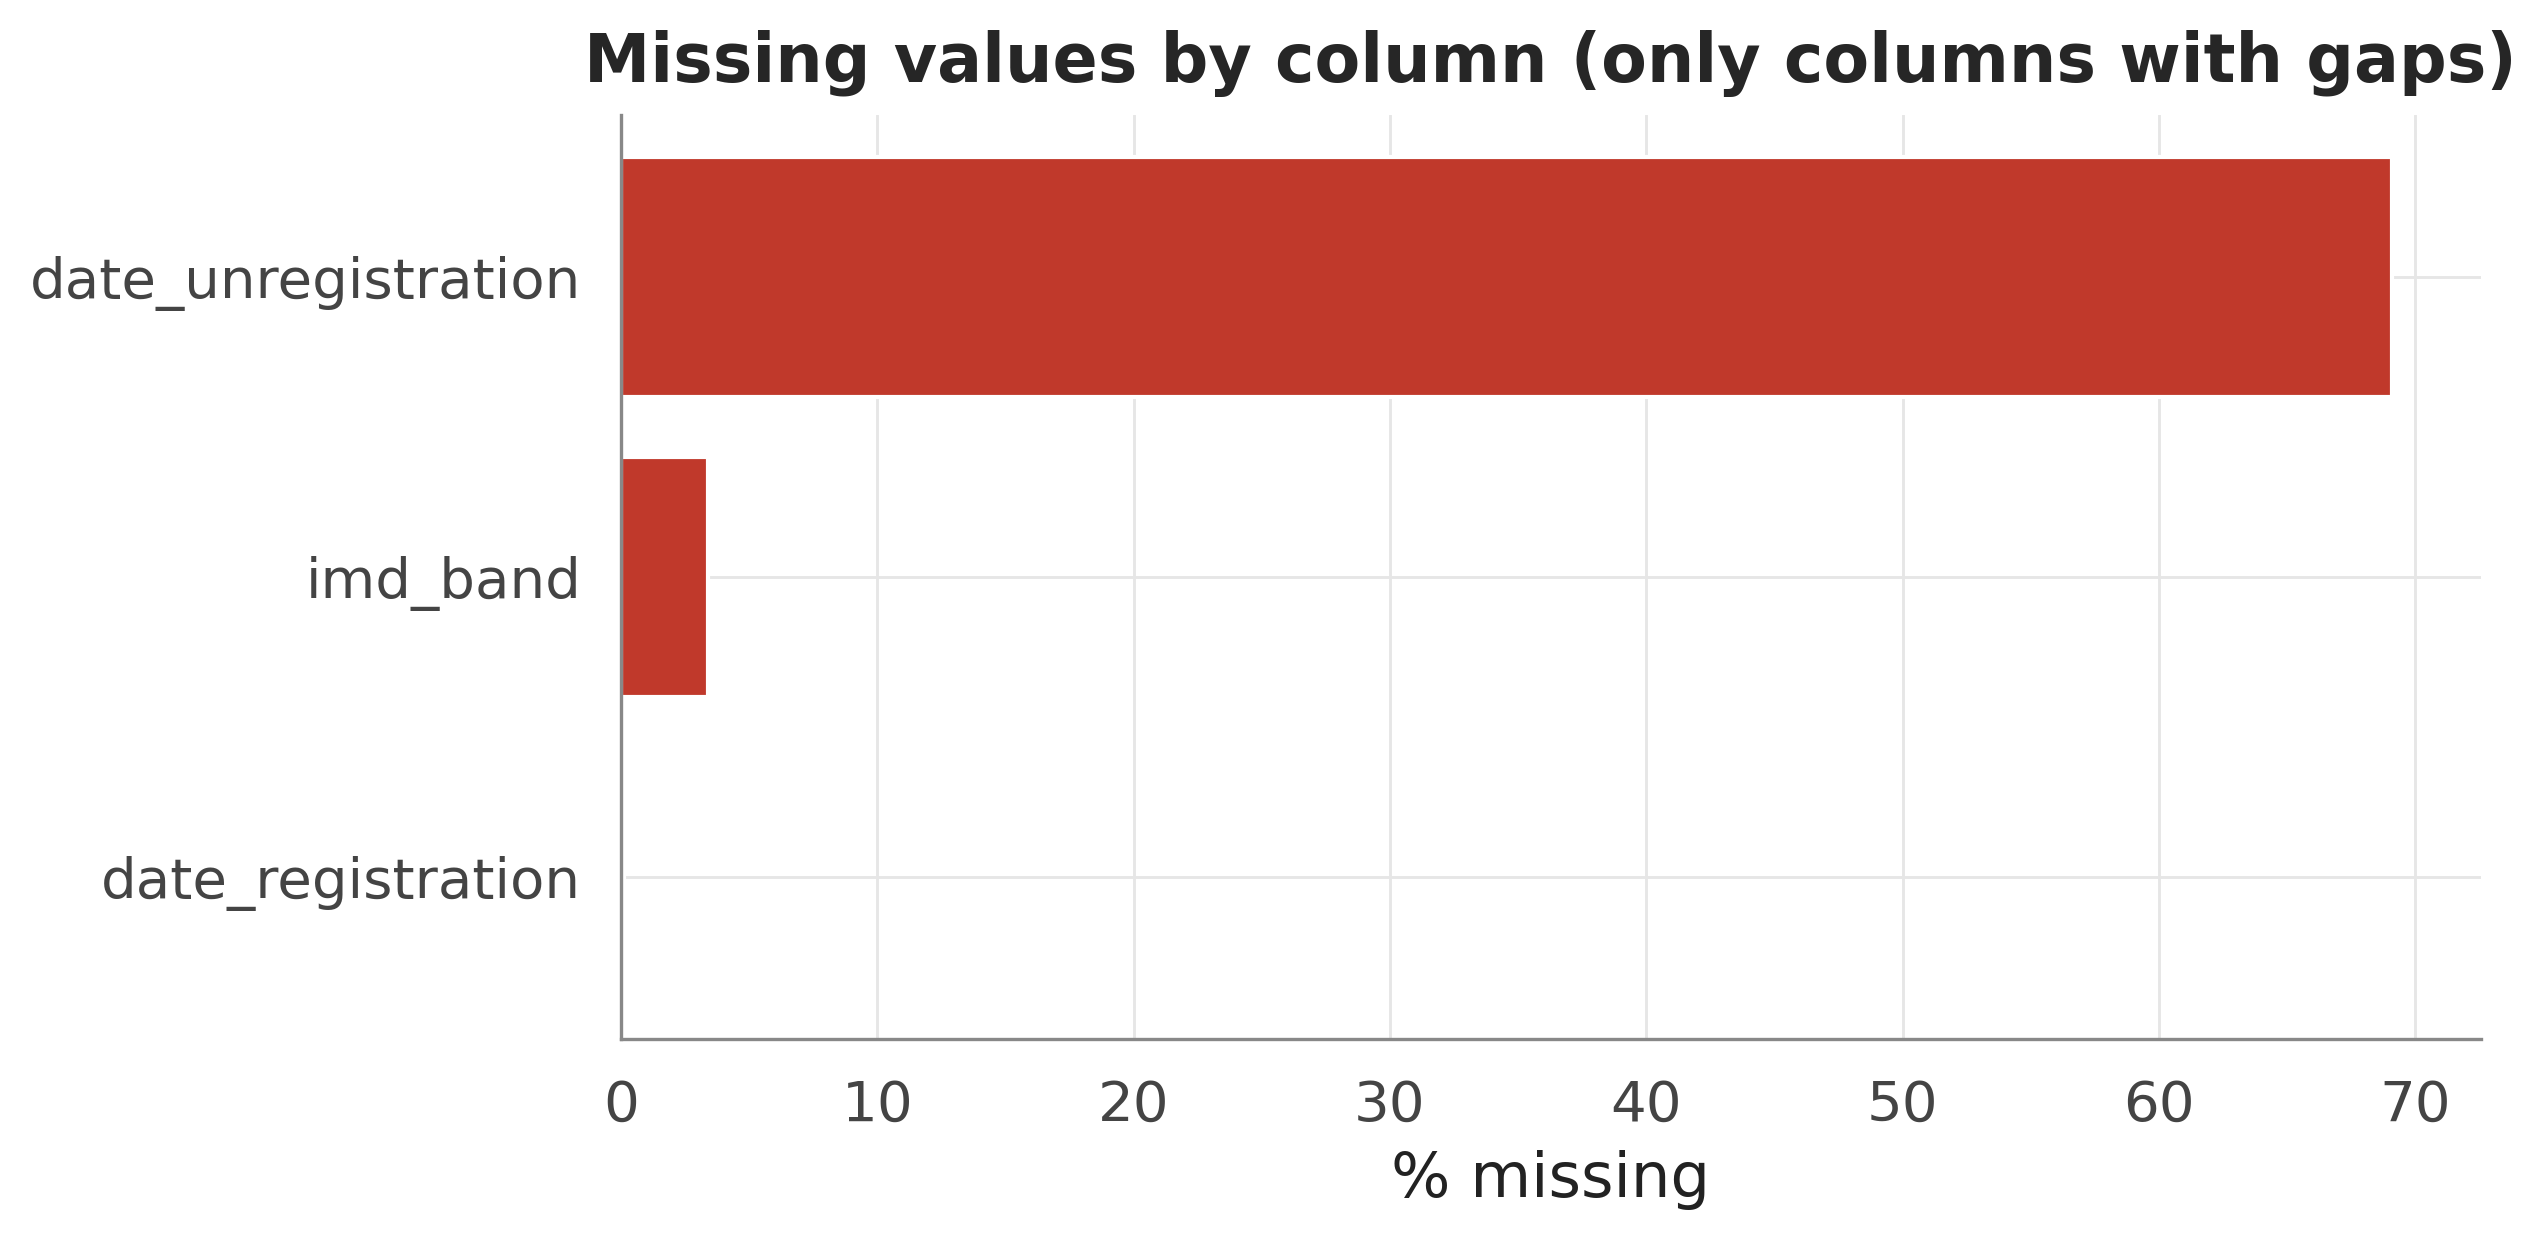
\includegraphics[width=\linewidth,height=0.66\textheight,keepaspectratio]{quality_missingness.png}\\
      {\scriptsize\itshape Missing values by column}
    \end{column}
  \end{columns}
\end{frame}

\begin{frame}{Duplicates \& Format Standardisation}
  \begin{itemize}\setlength\itemsep{0.4em}
    \item[\textcolor{cgreen}{\textbf{What}}]\, Duplicates: check the student–module–presentation key $\to$ \code{drop_duplicates} $\to$ 0 duplicate keys.
    \item[\textcolor{cgreen}{\textbf{What}}]\, Types: catalogue numeric / ordinal / nominal / binary / indicator (\code{VARIABLE_TYPES}).
    \item[\textcolor{cgreen}{\textbf{What}}]\, Standardise: strip text; reconcile dictionaries (region 13, education 5, imd\_band 10, age\_band 3, gender/disability 2).
    \item[\textcolor{cblue}{\textbf{Why}}]\, Correct types enable correct encoding in Part 4; standardising prevents `Y\,' $\neq$ `Y'.
    \item[\textcolor{themecol}{\textbf{Result}}]\, A dataset consistent in format \& type.
  \end{itemize}
\end{frame}

\begin{frame}{Outliers — Detection}
  \begin{columns}[T]
    \begin{column}{0.5\textwidth}
      \wwr{Logical checks (score $\in[0,100]$) + IQR-rule detection (\code{log_outliers}).}
          {Clickstream is strongly right-skewed: \code{clicks_resource} skew $\approx$ \textbf{34.7}, kurtosis $\approx$ \textbf{2{,}125}; \code{max_clicks_single_day} max = \textbf{6{,}988}.}
          {A 7-variable outlier table — handed off Binh $\to$ Duc.}
    \end{column}
    \begin{column}{0.5\textwidth}
      \centering
      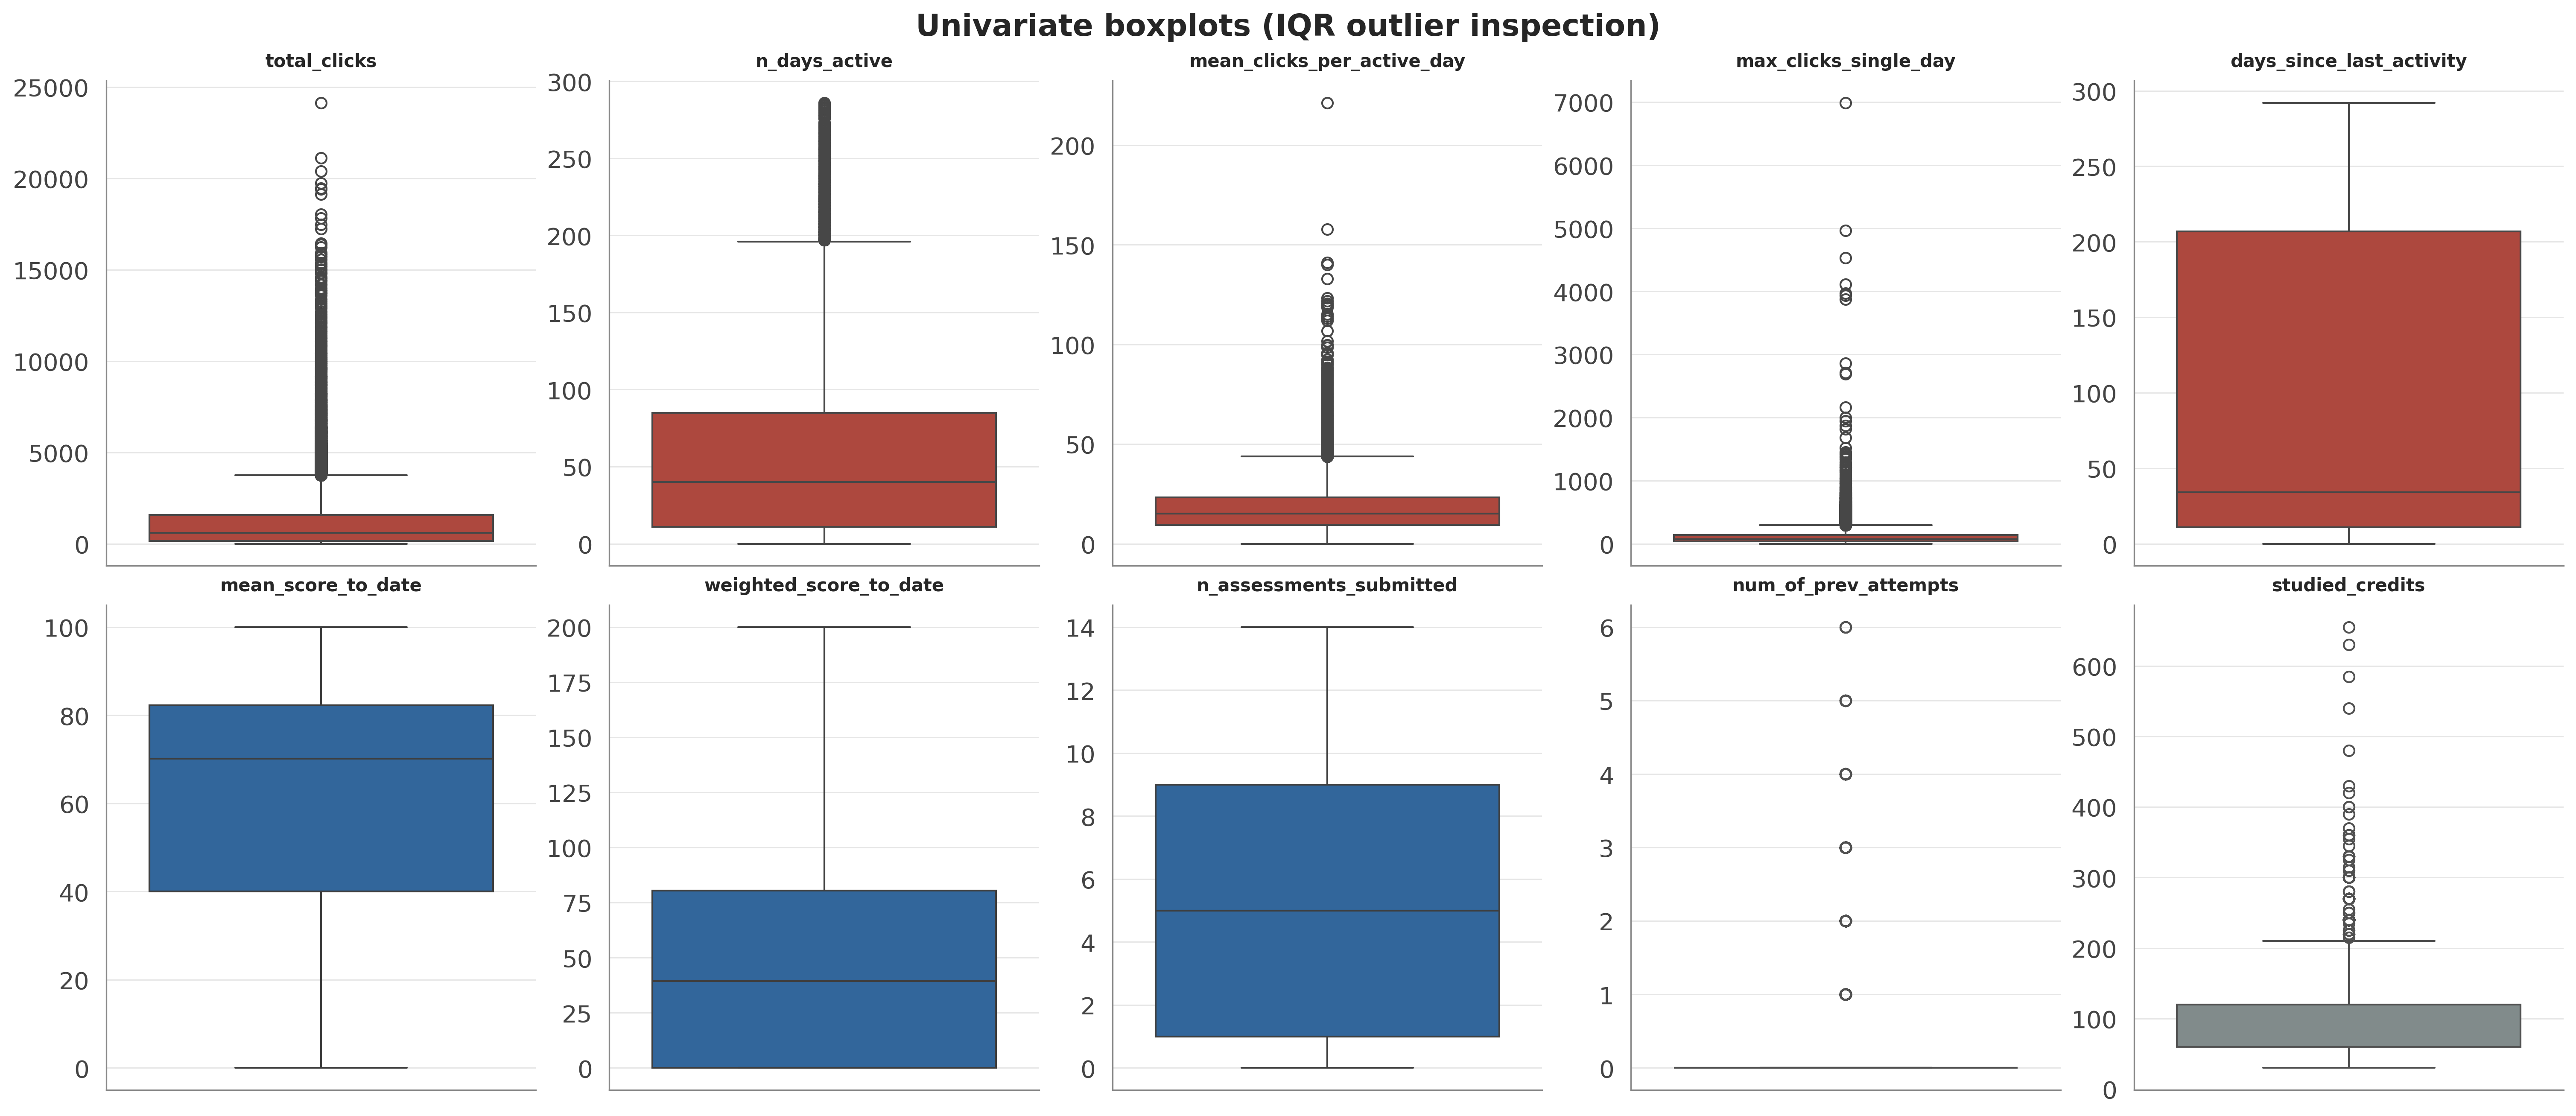
\includegraphics[width=\linewidth,height=0.72\textheight,keepaspectratio]{univariate_boxplots.png}\\
      {\scriptsize\itshape Univariate boxplots (IQR inspection)}
    \end{column}
  \end{columns}
\end{frame}

\begin{frame}{Outliers — Handling}
  \wwr{Per-variable strategy: \code{log1p} for 12 strongly-skewed click features · winsorise (clip 1\% each tail) for moderately skewed · none for naturally bounded.}
      {\textbf{No row is deleted}: an at-risk student's extreme values (e.g.\ many re-takes) are signal to keep.}
      {Every numeric feature is ``cleaner'' in distribution while all 32{,}593 rows remain.}
\end{frame}

\begin{frame}{Merge \& Final Clean Dataset}
  \wwr{Merge: studentInfo (base) $\leftarrow$ left join $\leftarrow$ registration $\leftarrow$ engagement $\leftarrow$ performance $\leftarrow$ courses.}
      {A before/after log proves no duplication, no loss (\code{validate='many_to_one'}).}
      {\code{master_raw} = 32{,}593 $\times$ 33 — clean, one row per student–module–presentation.}
  \vspace{2pt}
  {\footnotesize
  \setlength{\tabcolsep}{8pt}\renewcommand{\arraystretch}{1.2}
  \begin{tabularx}{\linewidth}{@{}Y r r@{}}
    \toprule
    \rowcolor{themecol}\hc{Step} & \hc{rows\_before} & \hc{rows\_after}\\
    \midrule
    studentInfo (base) & 32{,}593 & 32{,}593\\
    \rowcolor{rowtint}+ registration & 32{,}593 & 32{,}593\\
    + engagement & 32{,}593 & 32{,}593\\
    \rowcolor{rowtint}+ performance & 32{,}593 & 32{,}593\\
    \bottomrule
  \end{tabularx}}
\end{frame}

% ===================================================================== EDA
\partframe{}{Exploratory Data Analysis}{Duc}

\begin{frame}{EDA Objectives}
  \begin{itemize}\setlength\itemsep{0.4em}
    \item Understand the data: 32{,}593 students, 33 variables (demographic · engagement · assessment).
    \item Check quality: missing data, types, outliers.
    \item Find features that separate at-risk vs not-at-risk students.
    \item Serve two decisions: \textbf{feature selection} \& \textbf{leakage control}.
  \end{itemize}
  \keynum{32{,}593 records · 33 columns · 3 feature groups.}
\end{frame}

\begin{frame}{Univariate Analysis}
  \begin{columns}[T]
    \begin{column}{0.46\textwidth}
      \wwr{Histogram + KDE and boxplots per numeric feature.}
          {Most clickstream features are \textbf{strongly right-skewed}; heavy tails are \textbf{real} outliers (super-active students), not removed.}
          {$\Rightarrow$ log transform + standardisation; use non-parametric tests.}
      \keynum{\code{clicks_resource} skew \textbf{34.71} · kurtosis \textbf{2{,}125.45}.}
    \end{column}
    \begin{column}{0.54\textwidth}
      \centering
      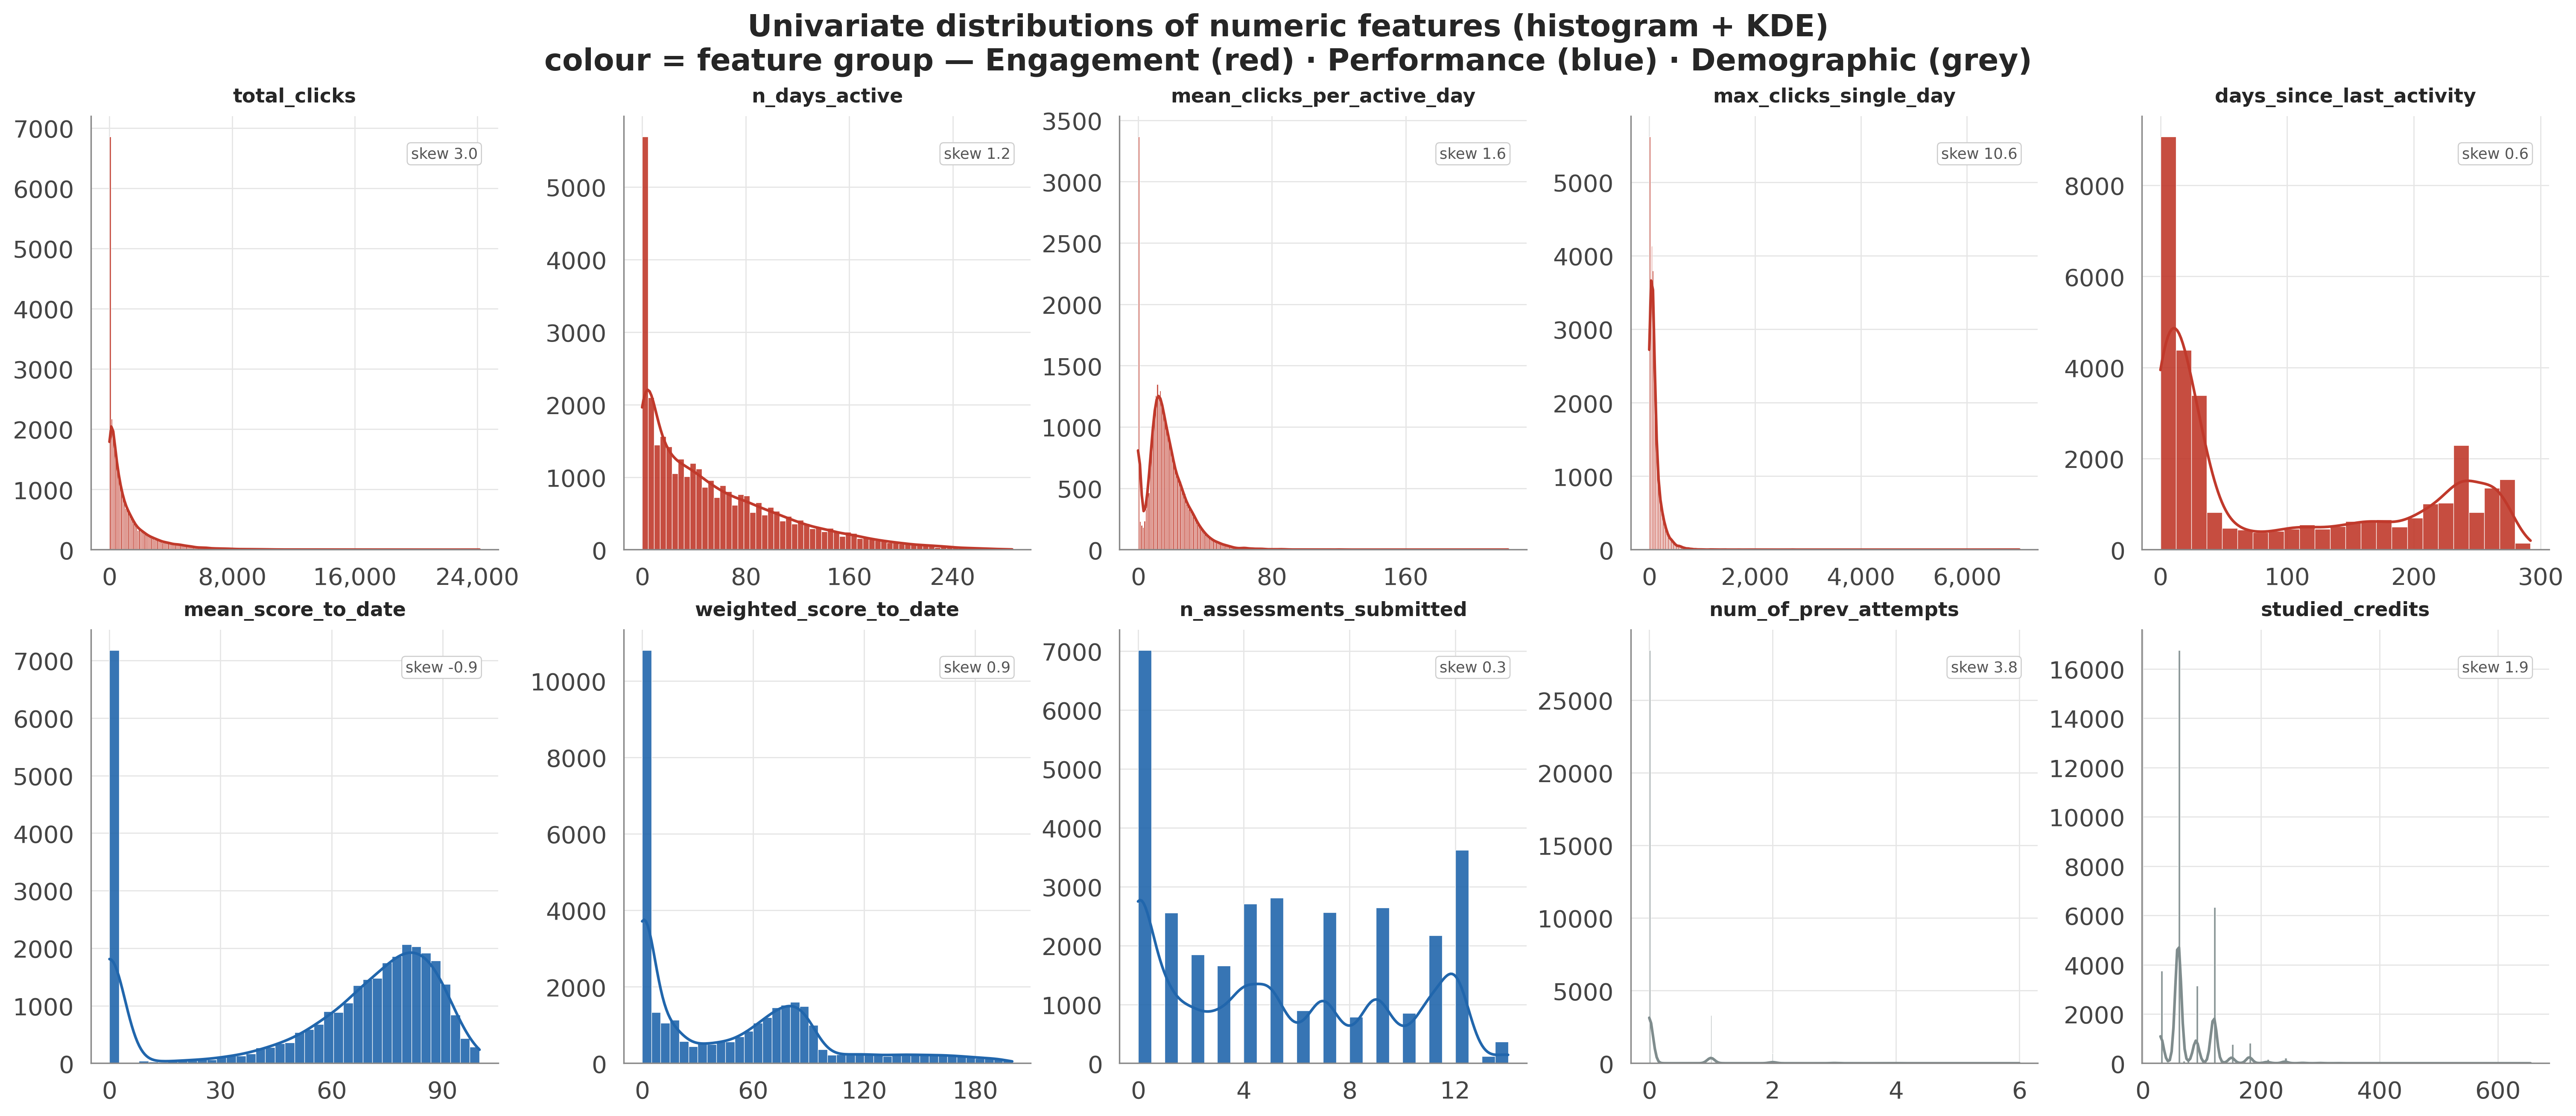
\includegraphics[width=\linewidth,height=0.74\textheight,keepaspectratio]{univariate_hist_kde.png}
    \end{column}
  \end{columns}
\end{frame}

\begin{frame}{Bivariate Analysis (vs at-risk)}
  \begin{columns}[T]
    \begin{column}{0.5\textwidth}
      \wwr{Compare the two classes with \textbf{Cohen's d} + Mann–Whitney (BH-corrected).}
          {At n$\approx$32k p-values are tiny $\to$ rank by \textbf{effect size}, not p.}
          {Top: \code{days_since_last_activity} d=\textbf{2.55} · \code{n_assessments_submitted} 2.05 · \code{weighted_score_to_date} 1.96. \textbf{19/19} features significant.}
      \keynum{days\_since: 171 vs 14 days · n\_assessments: 2.3 vs 8.6.}
    \end{column}
    \begin{column}{0.5\textwidth}
      \centering
      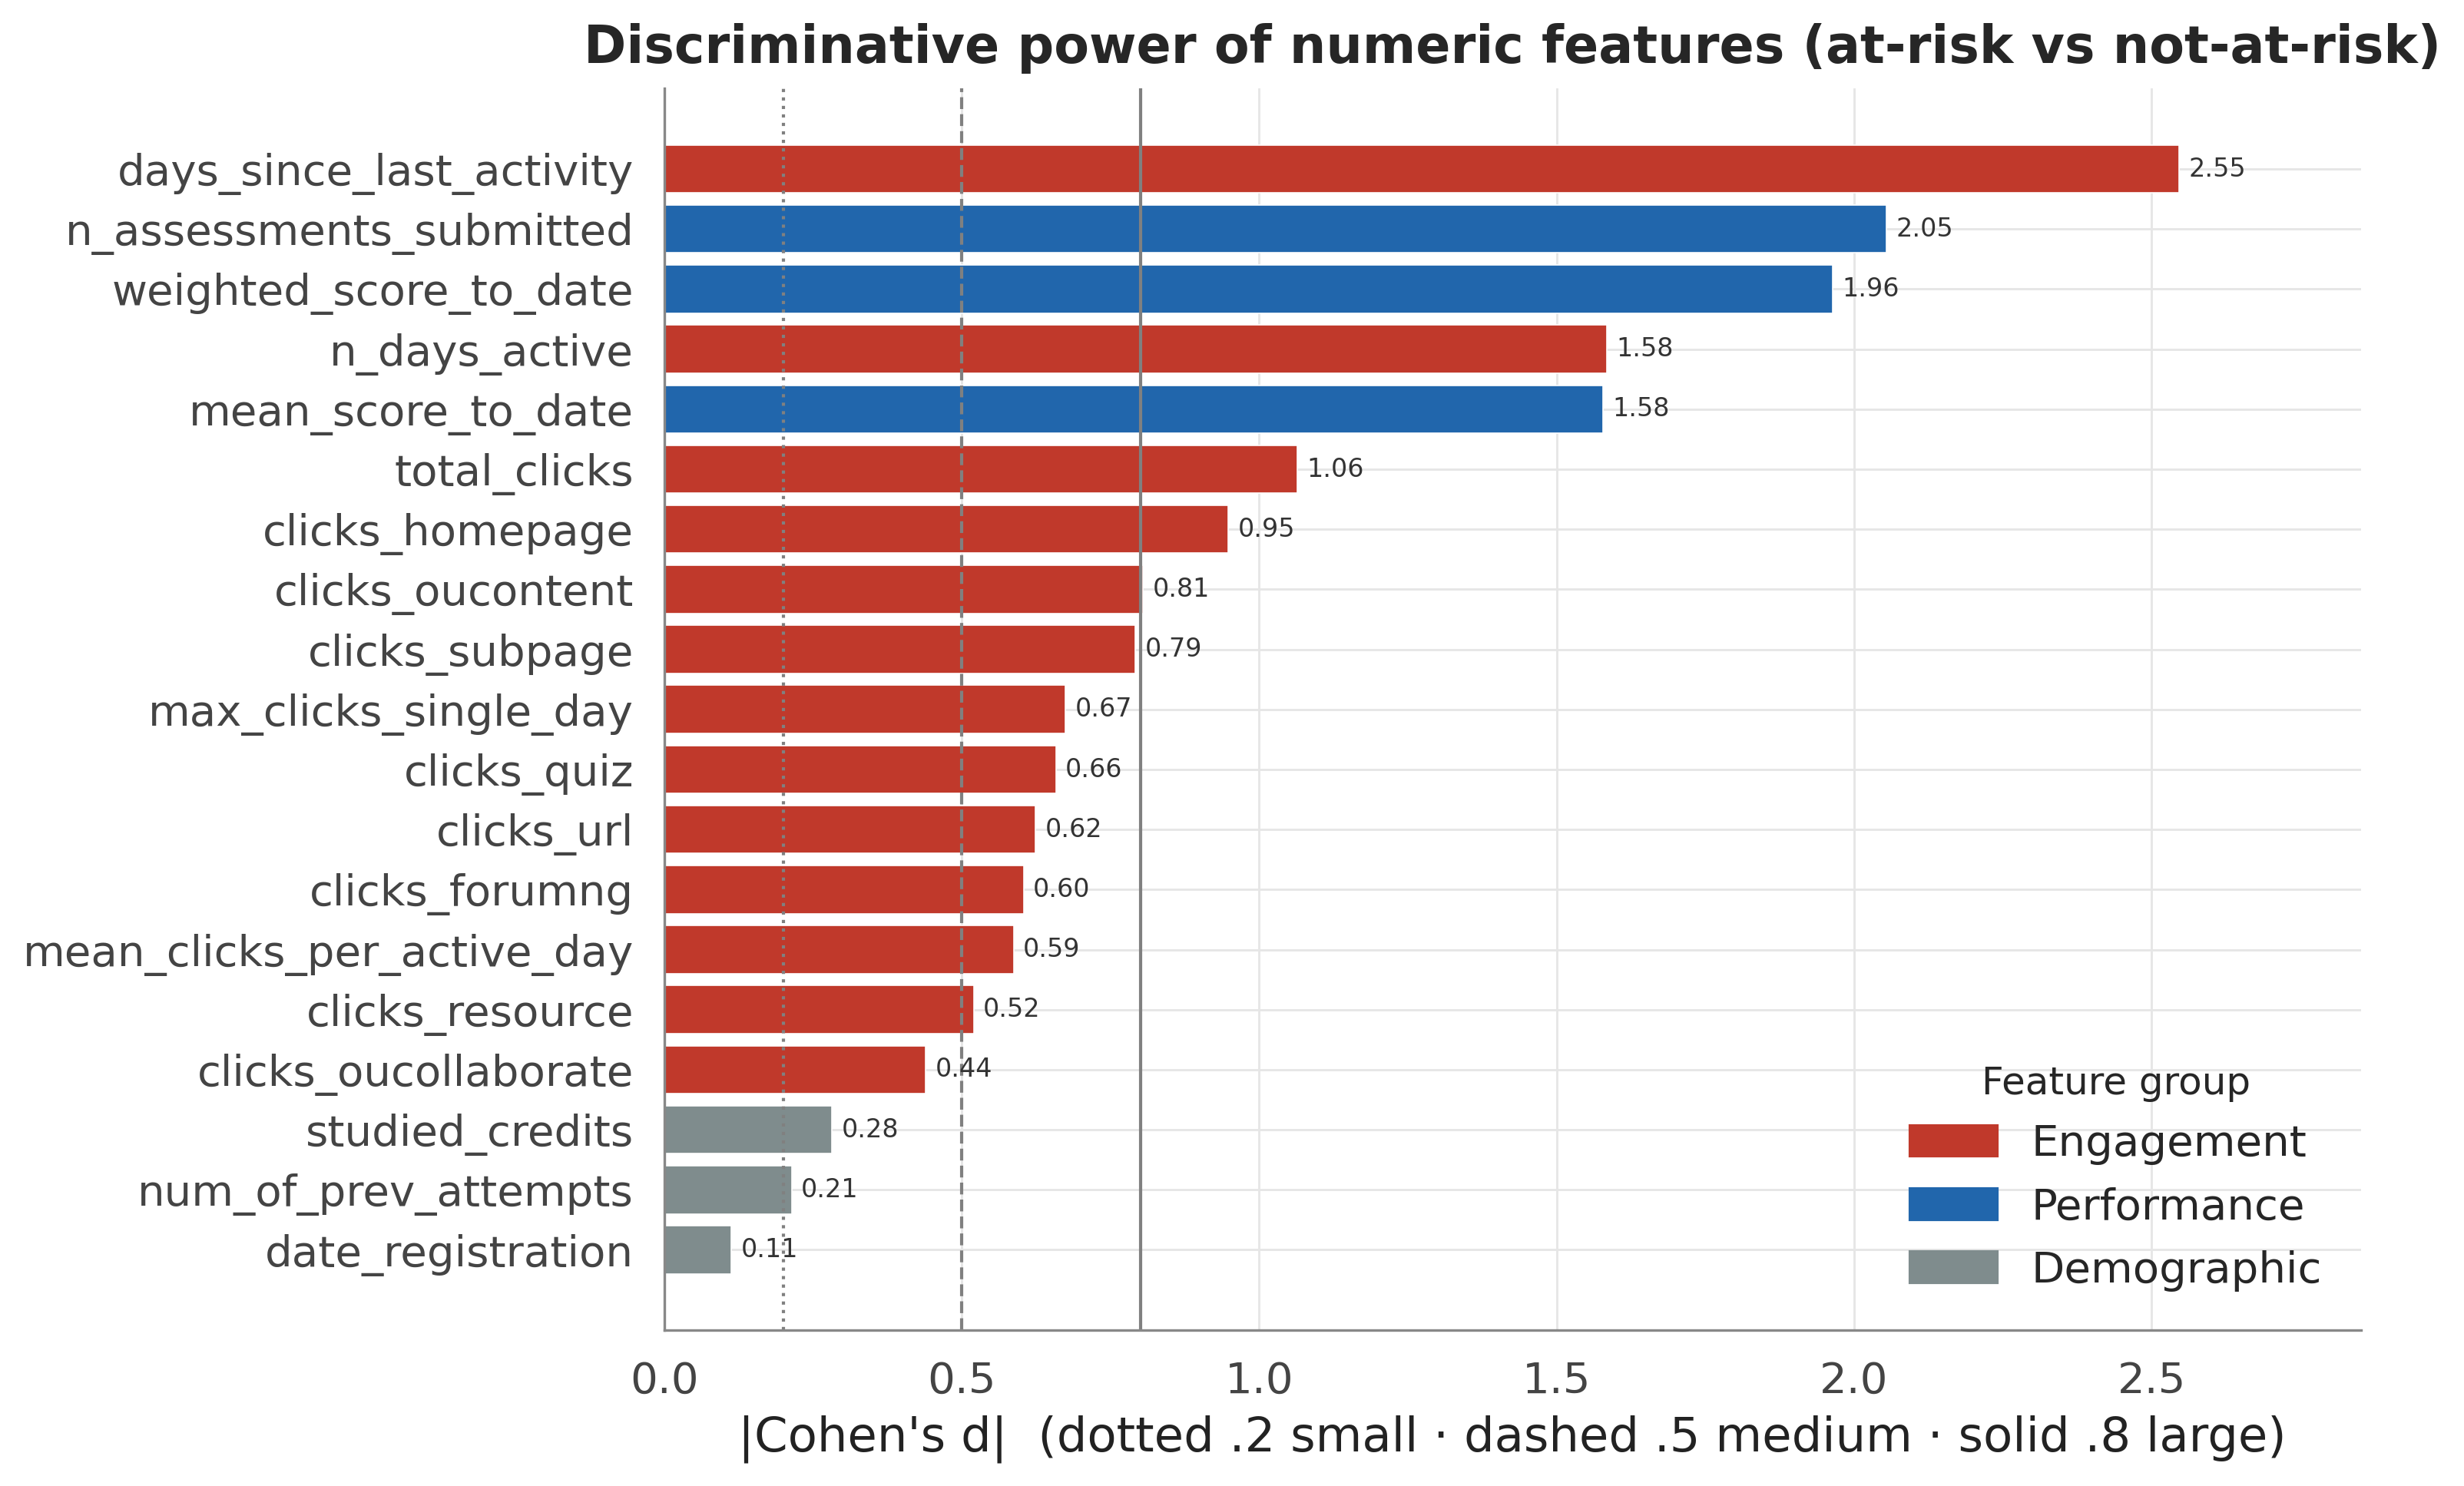
\includegraphics[width=\linewidth,height=0.74\textheight,keepaspectratio]{bivariate_effect_sizes.png}
    \end{column}
  \end{columns}
\end{frame}

\begin{frame}{Multivariate — Correlation \& Leakage Check}
  \begin{columns}[T]
    \begin{column}{0.5\textwidth}
      \wwr{Pearson (linear) + Spearman (monotonic) heatmaps; correlation with the label; leakage check.}
          {Leakage is a \textbf{mandatory} step — a feature with |r|$\geq$0.95 vs the label is suspicious.}
          {Top |r| with label: \code{days_since} +0.78 · \code{n_assessments} $-$0.72 · \code{weighted_score} $-$0.71. \textbf{No feature |r|$\geq$0.95} $\Rightarrow$ no leakage.}
      \keynum{max r(label) = 0.78 · leakage $\geq$0.95: 0 · Cramér's V $\leq$ 0.15.}
    \end{column}
    \begin{column}{0.5\textwidth}
      \centering
      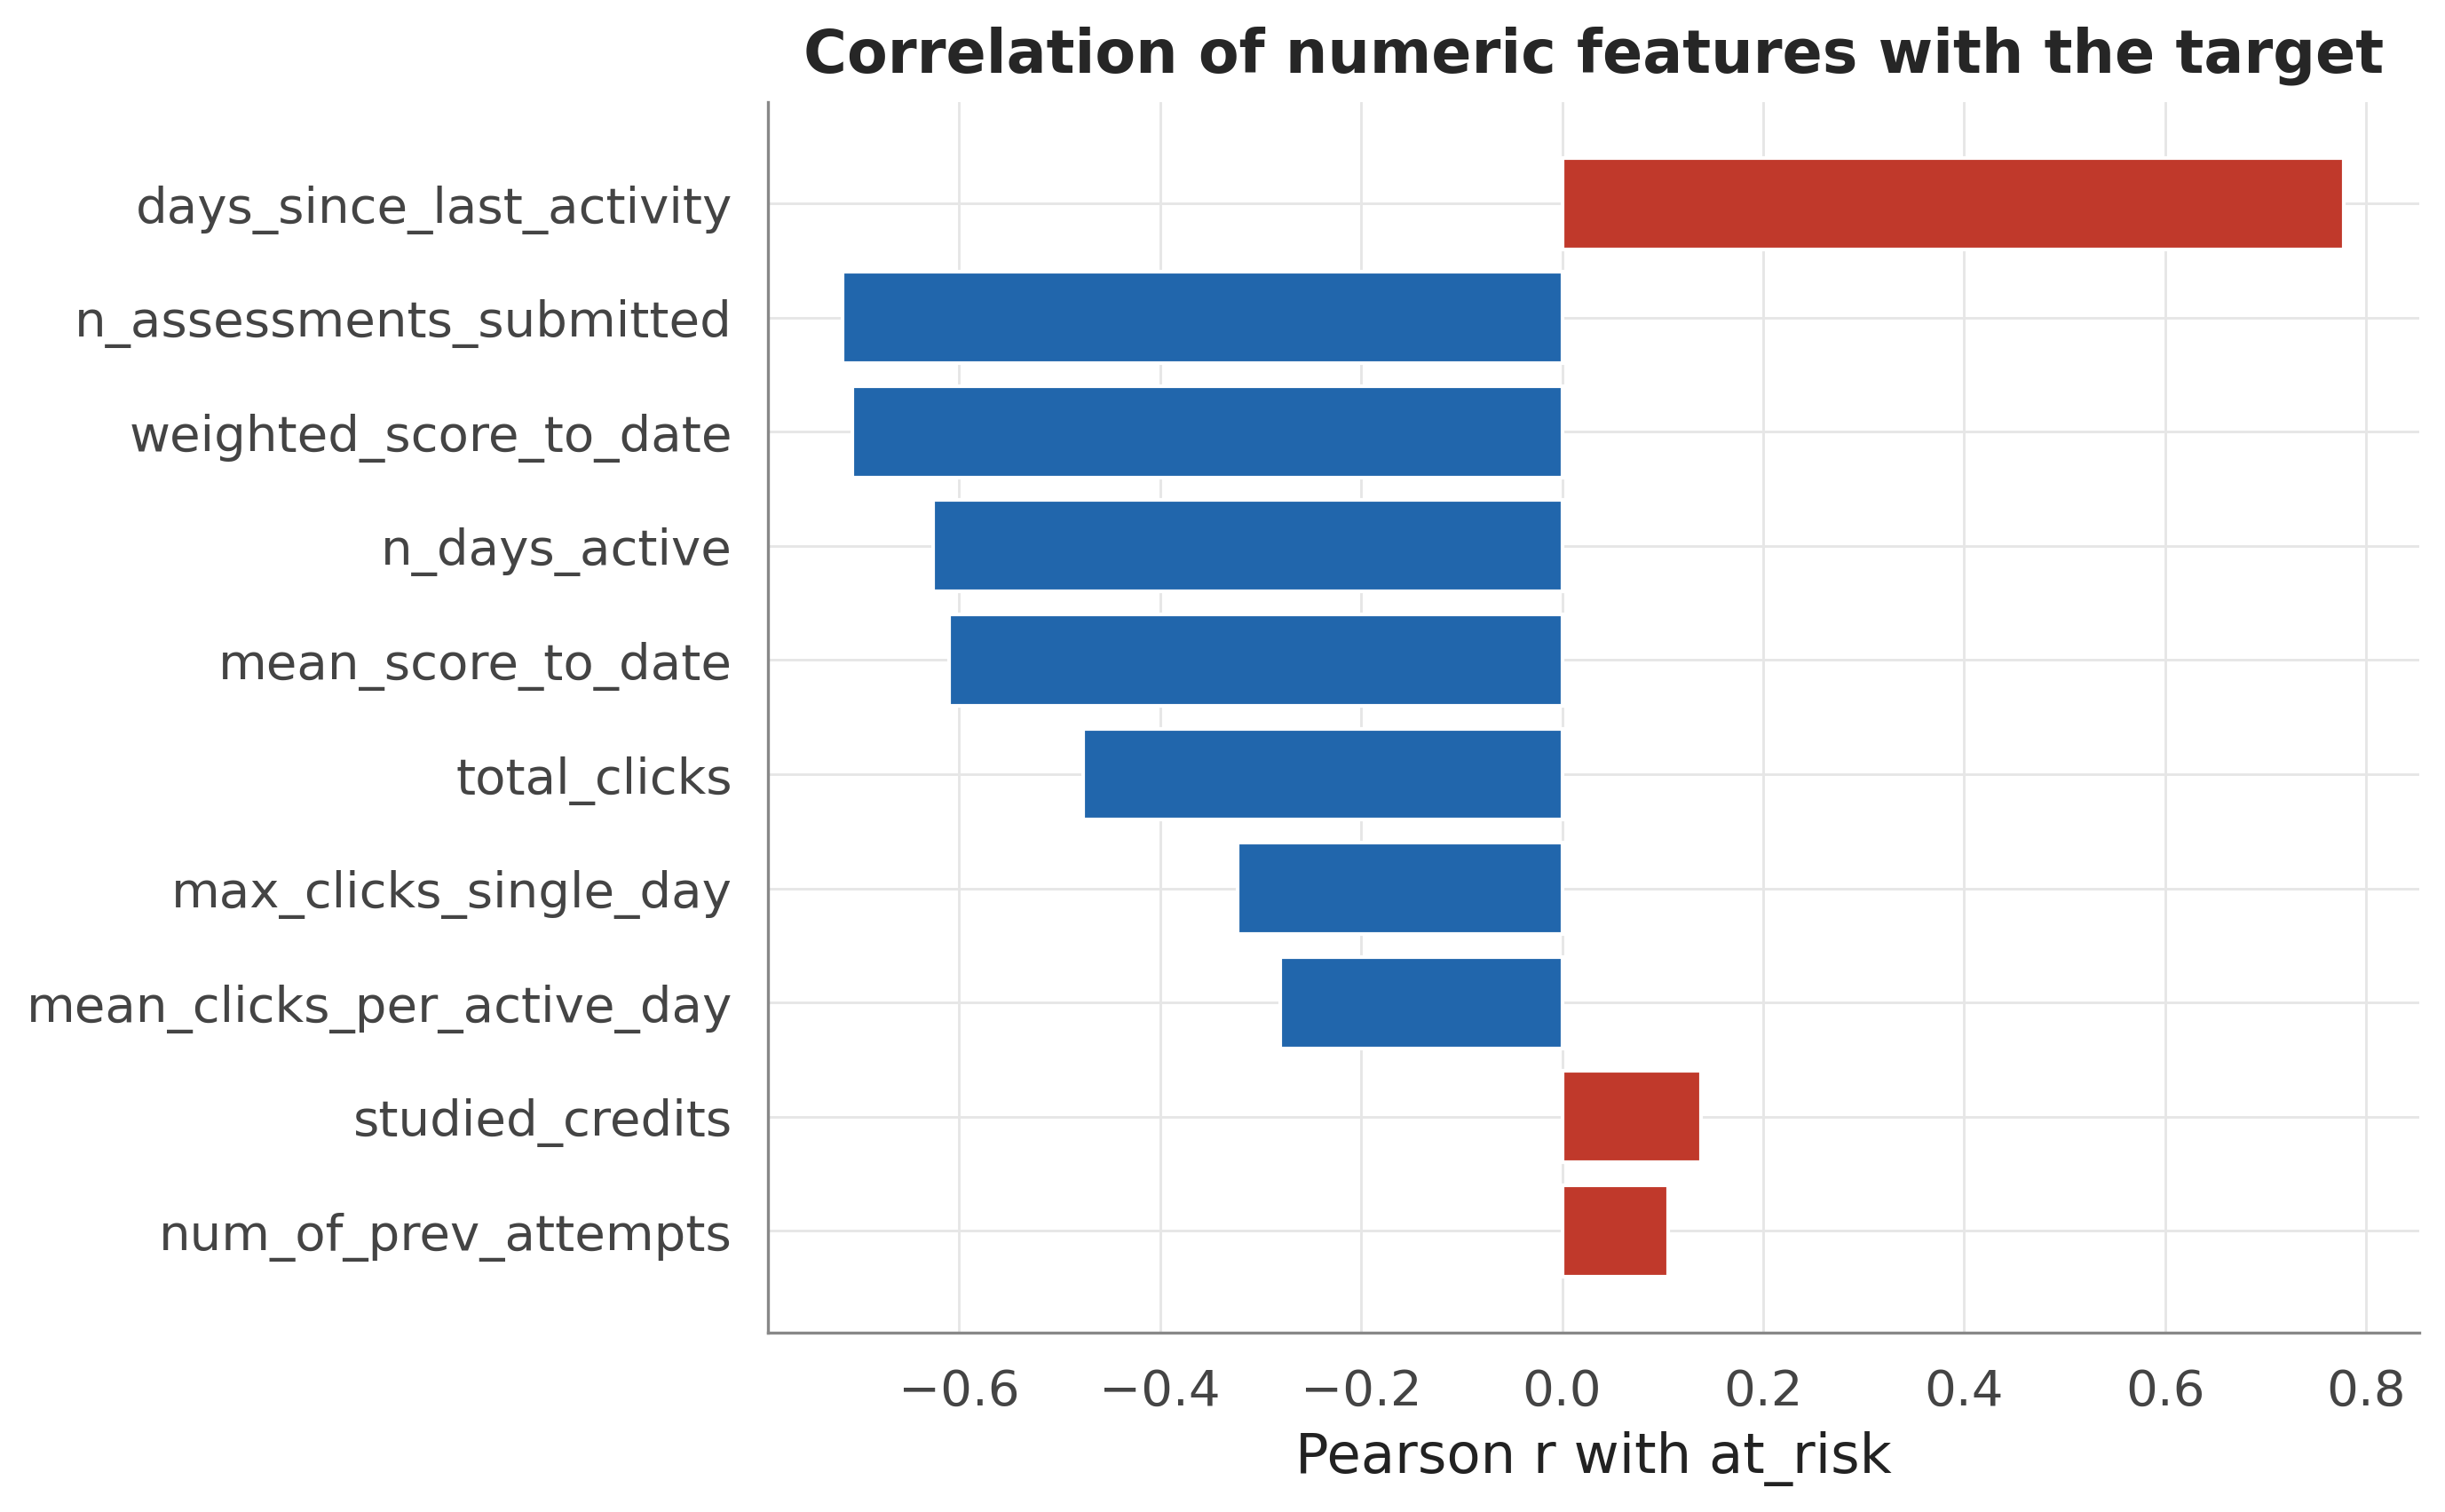
\includegraphics[width=\linewidth,height=0.72\textheight,keepaspectratio]{corr_with_target.png}
    \end{column}
  \end{columns}
\end{frame}

\begin{frame}{Time-Aware Analysis \& EDA Conclusion (RQ1)}
  \begin{columns}[T]
    \begin{column}{0.5\textwidth}
      \wwr{Measure Cohen's d per feature at 6 checkpoints 10\%$\to$100\%; signal grows steadily.}
          {First to reach d$\geq$0.8: \code{n_days_active} \textbf{and} \code{days_since_last_activity} from \textbf{10\%}; scores/submissions from \textbf{20\%}.}
          {Early prediction feasible from \textbf{$\sim$10–20\%} of the course; prioritise engagement + assessment features.}
      \keynum{weighted\_score d: 0.61$\to$1.96 · n\_assessments: 0.67$\to$2.05 (10\%$\to$100\%).}
    \end{column}
    \begin{column}{0.5\textwidth}
      \centering
      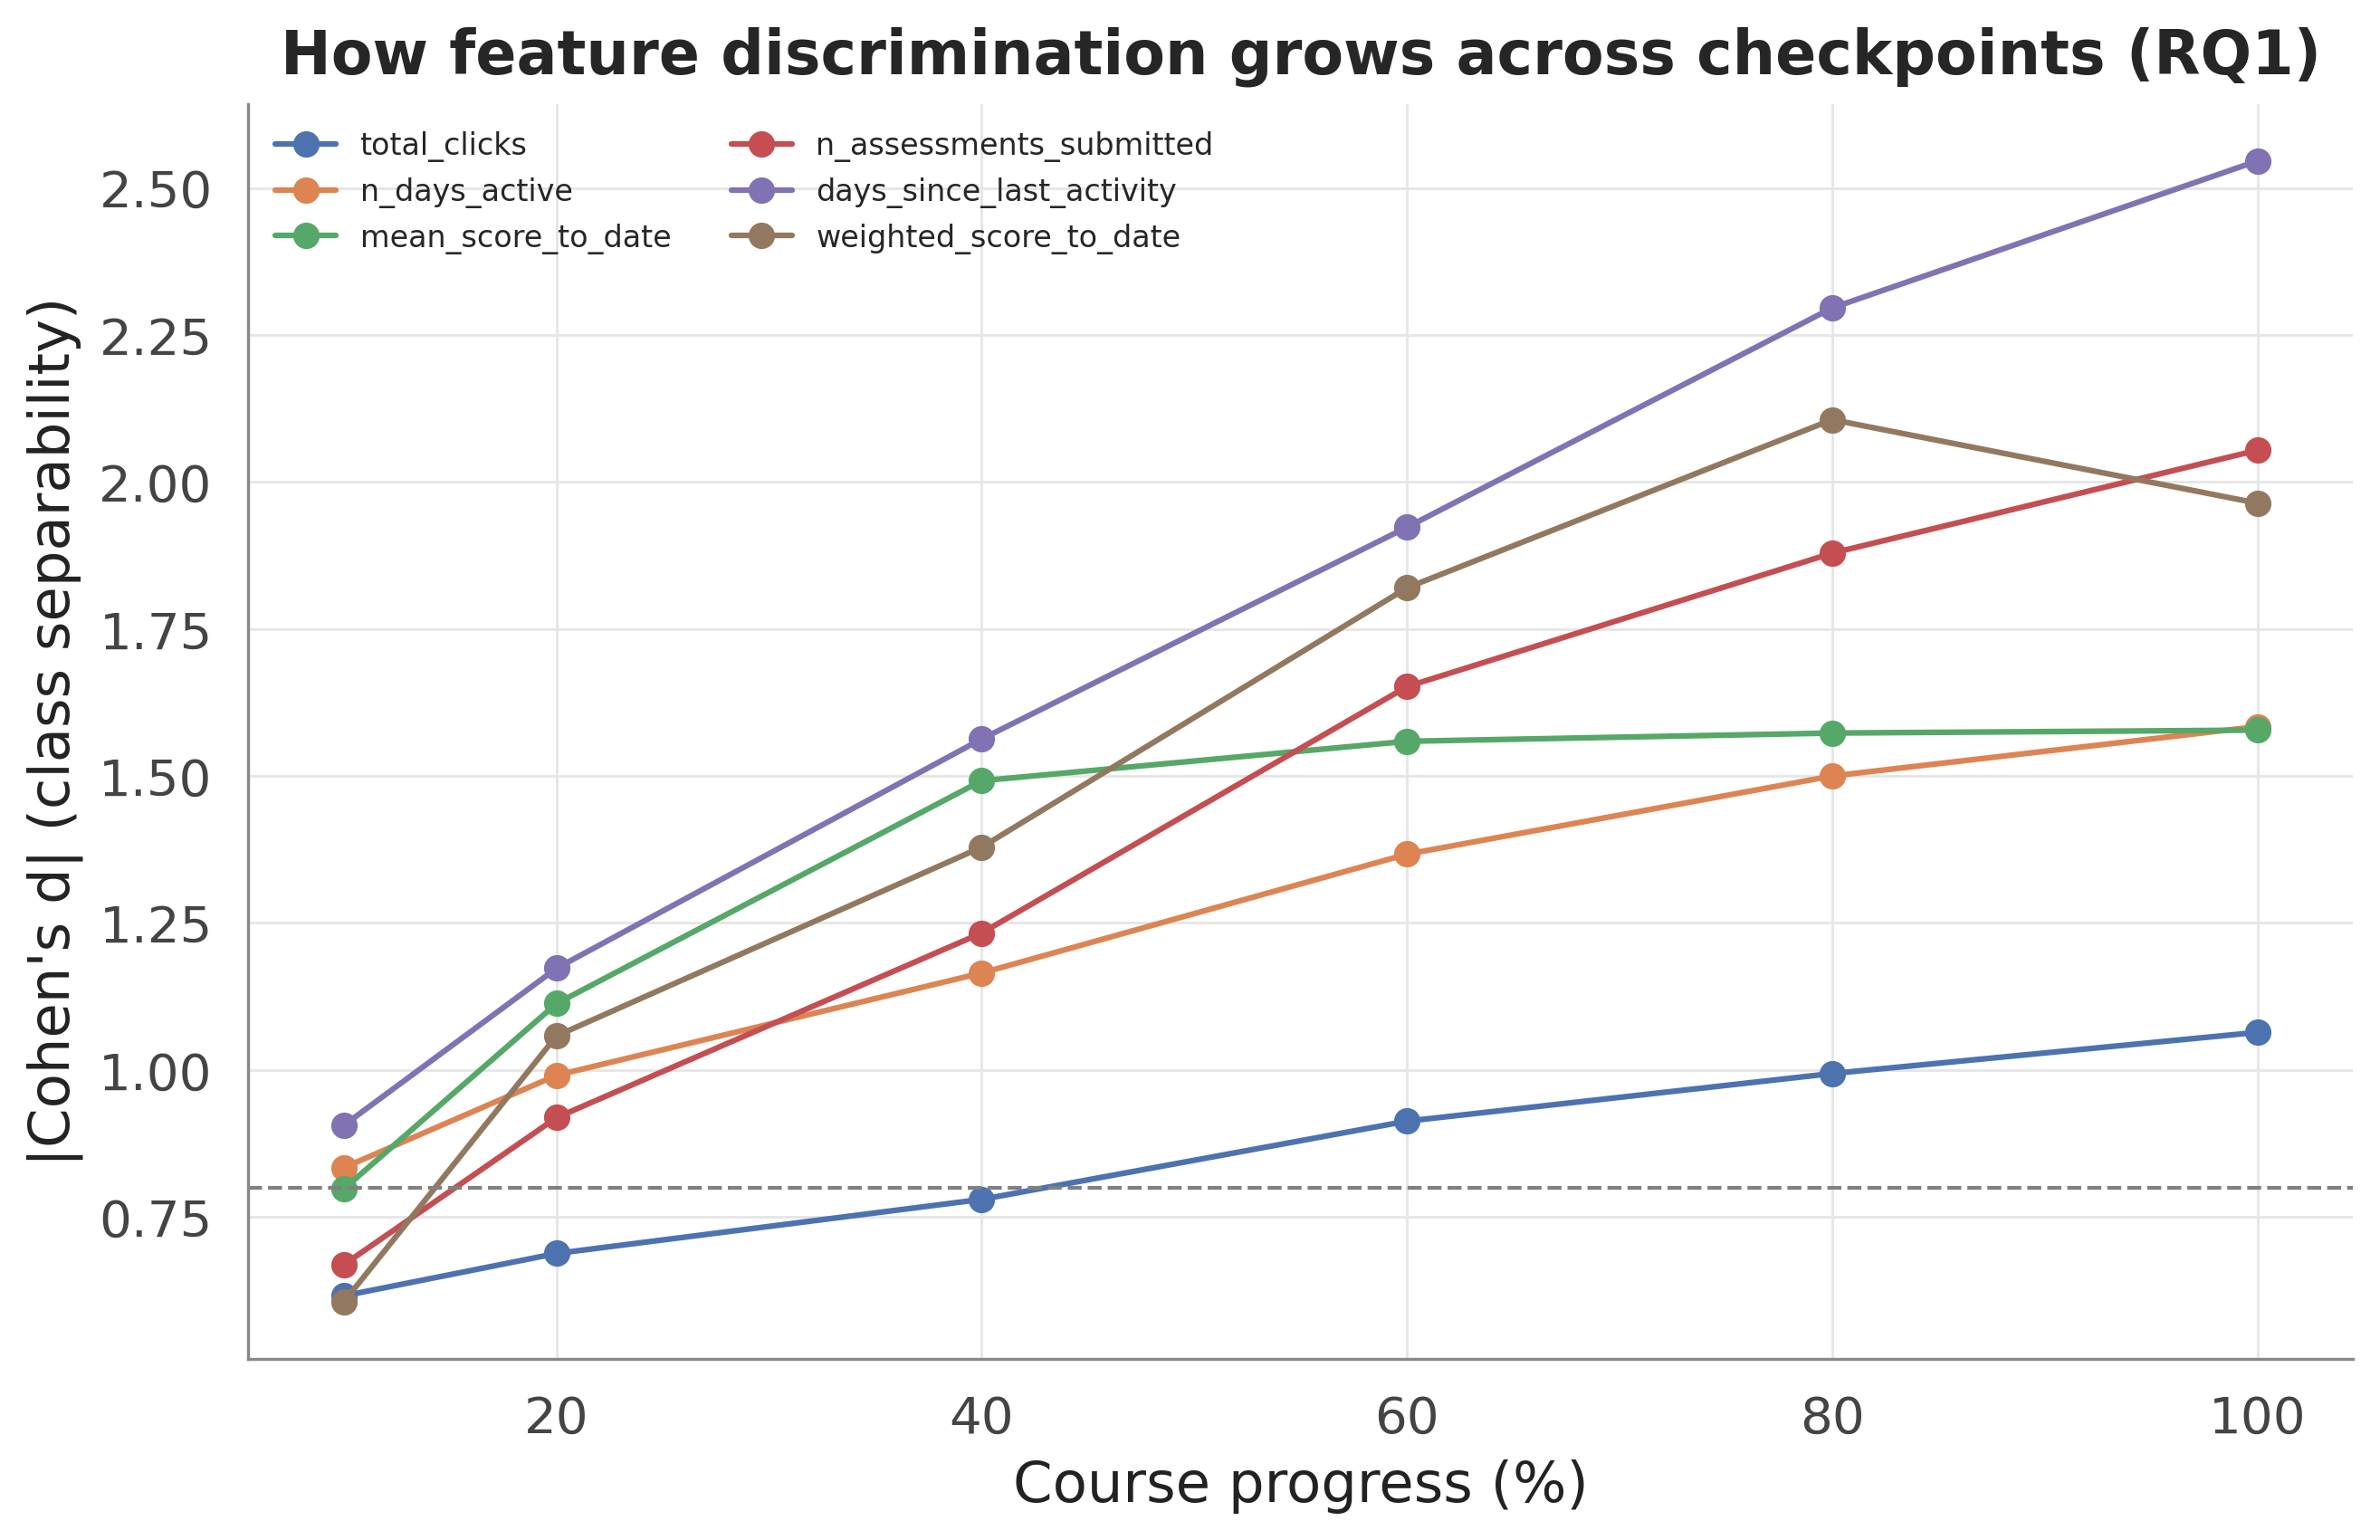
\includegraphics[width=\linewidth,height=0.72\textheight,keepaspectratio]{time_discrimination_curve.png}
    \end{column}
  \end{columns}
\end{frame}

% ===================================================================== PART 4
\partframe{4}{Transformation \& Standardisation}{Binh}

\begin{frame}{Encoding Categorical Variables}
  \wwr{Four strategies by variable nature (see table).}
      {Wrong encoding (one-hot for an ordinal) \textbf{destroys} the order information.}
      {Text $\to$ numeric; readable by both model and XAI.}
  \vspace{2pt}
  {\footnotesize
  \setlength{\tabcolsep}{6pt}\renewcommand{\arraystretch}{1.25}
  \begin{tabularx}{\linewidth}{@{}l Y l@{}}
    \toprule
    \rowcolor{themecol}\hc{Kind} & \hc{Variables} & \hc{Method}\\
    \midrule
    Ordinal & \code{highest_education}, \code{imd_band}, \code{age_band} & OrdinalEncoder\\
    \rowcolor{rowtint}Nominal & \code{region}, \code{code_module}, \code{code_presentation} & OneHotEncoder\\
    Binary & \code{gender}, \code{disability} & BinaryEncoder (0/1)\\
    \rowcolor{rowtint}Indicator & \code{not_submitted} & passthrough\\
    \bottomrule
  \end{tabularx}}
\end{frame}

\begin{frame}{Skew Transformation (\code{log1p})}
  \begin{columns}[T]
    \begin{column}{0.5\textwidth}
      \wwr{Apply \code{log1p} to the strongly right-skewed click features (from Part 3).}
          {Reduce heavy tails $\to$ stabilise linear/distance models; evidence: skew $\sim$13–35 in EDA.}
          {Click features become more balanced, no rows lost.}
    \end{column}
    \begin{column}{0.5\textwidth}
      \centering
      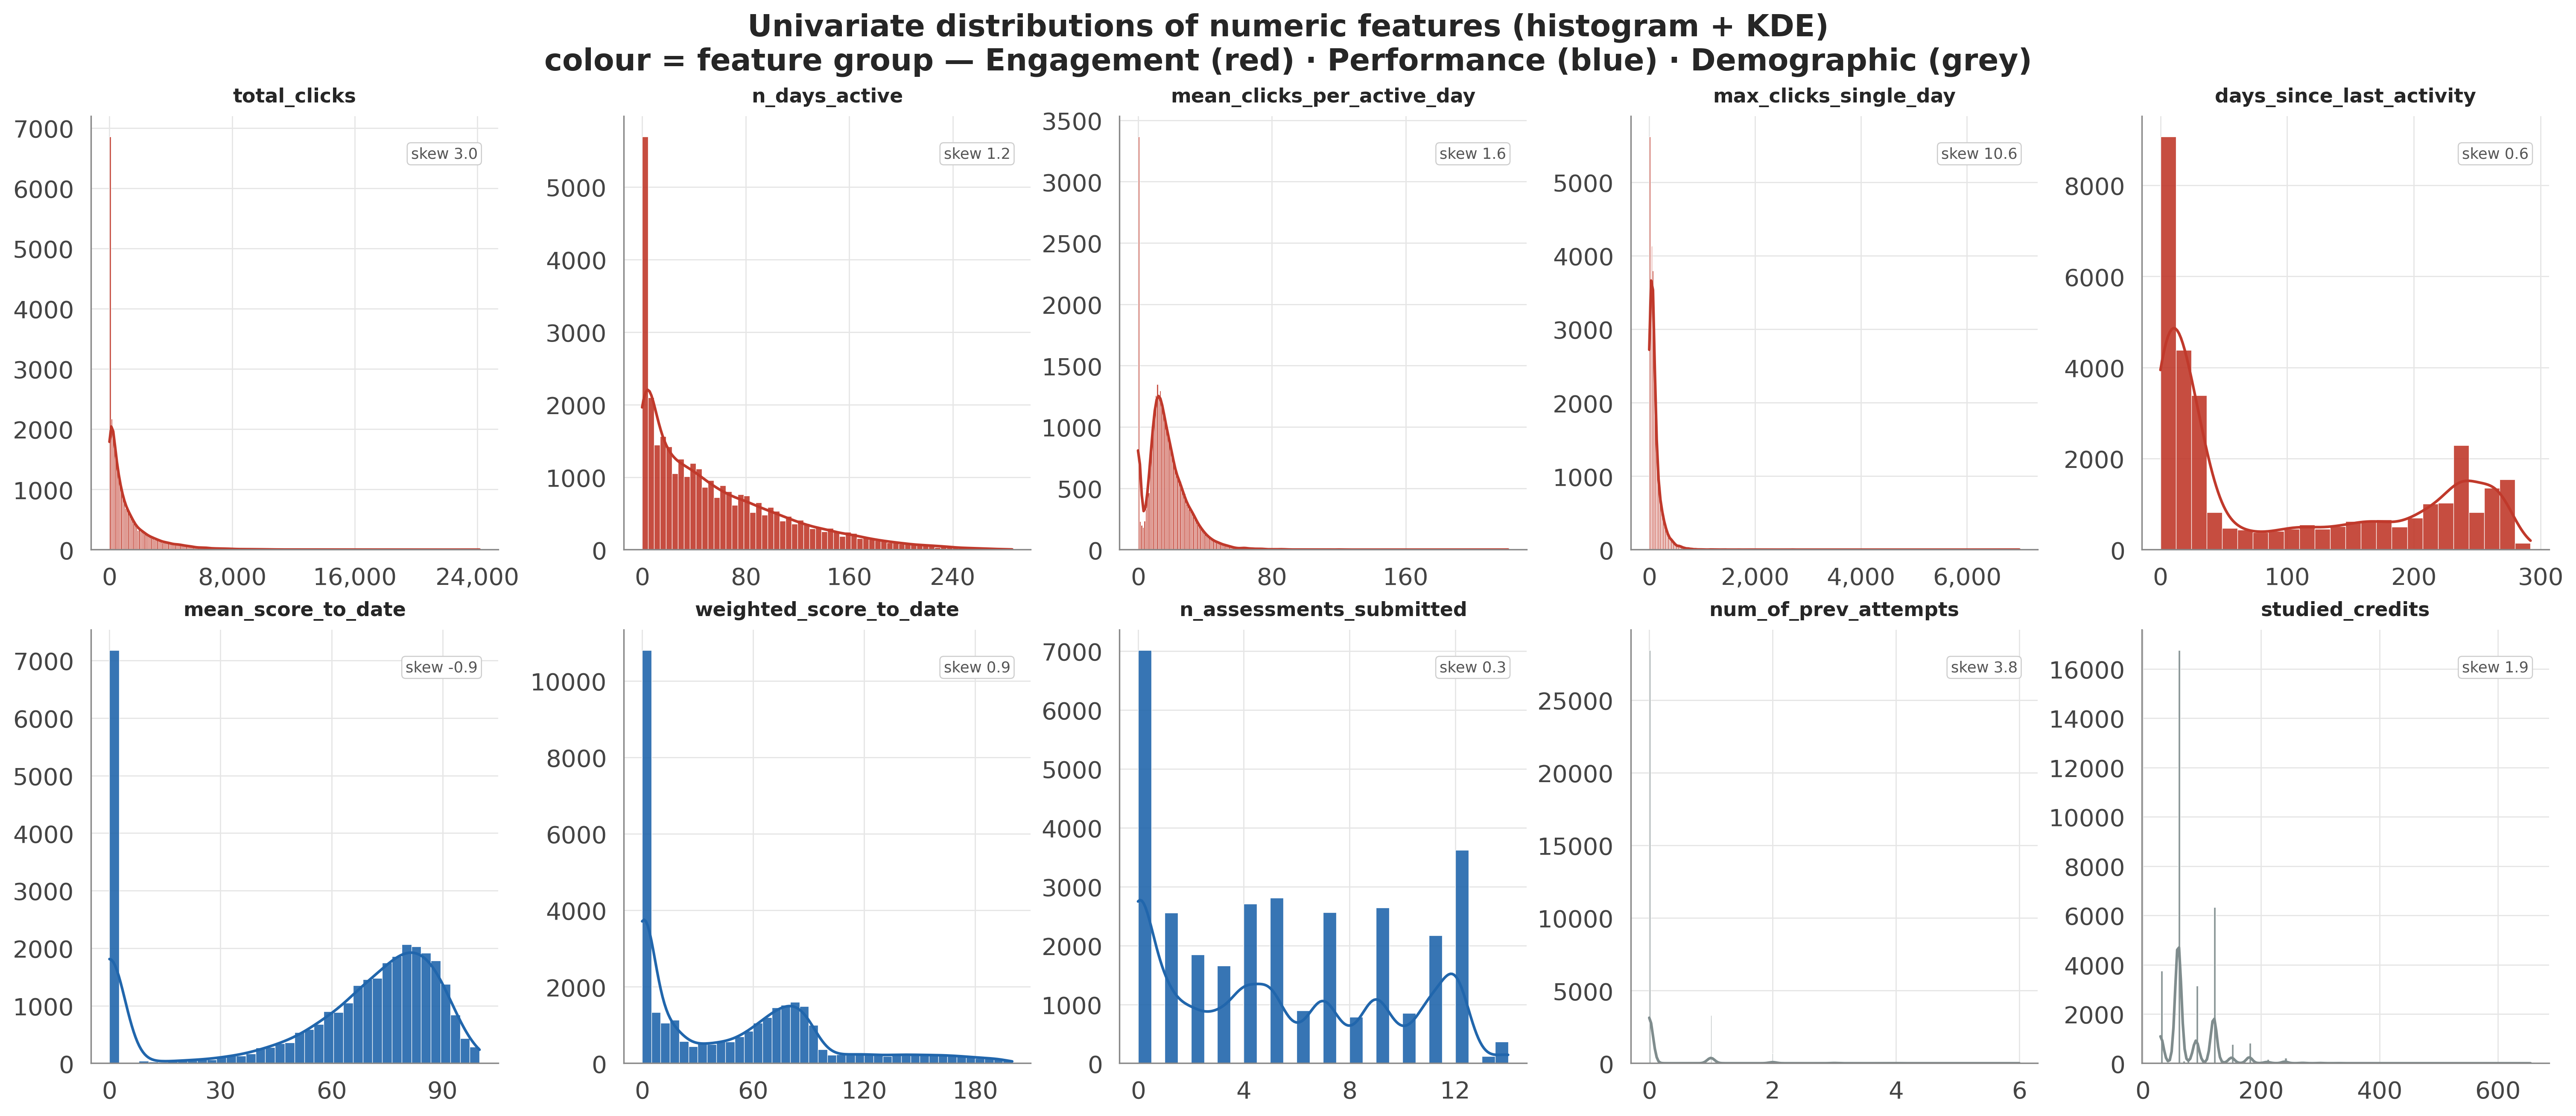
\includegraphics[width=\linewidth,height=0.72\textheight,keepaspectratio]{univariate_hist_kde.png}\\
      {\scriptsize\itshape Right-skew $\to$ log1p}
    \end{column}
  \end{columns}
\end{frame}

\begin{frame}{Scaling (StandardScaler)}
  \wwr{\code{StandardScaler} brings numeric features to mean 0, std 1.}
      {Total clicks (0–thousands) overwhelm scores (0–100) $\to$ mandatory for Logistic Regression \& ANN.}
      {Fit on \textbf{train only}, transform both train/test (\code{scaler.mean_} computed from train).}
\end{frame}

\begin{frame}{Feature Creation \& Significance}
  \begin{columns}[T]
    \begin{column}{0.5\textwidth}
      \wwr{Engagement: \code{total_clicks}, \code{n_days_active}, 8$\times$\code{clicks_<type>}, max/mean clicks, \code{days_since_last_activity}. Assessment: \code{mean_score_to_date}, \code{weighted_score_to_date}, \code{n_assessments_submitted}, \code{not_submitted}.}
          {Each feature carries a hypothesis: ``long inactivity / missed submissions $\Rightarrow$ higher risk''.}
          {Validated by |Cohen's d|: days\_since 2.55 · n\_assessments 2.05 · weighted\_score 1.96.}
    \end{column}
    \begin{column}{0.5\textwidth}
      \centering
      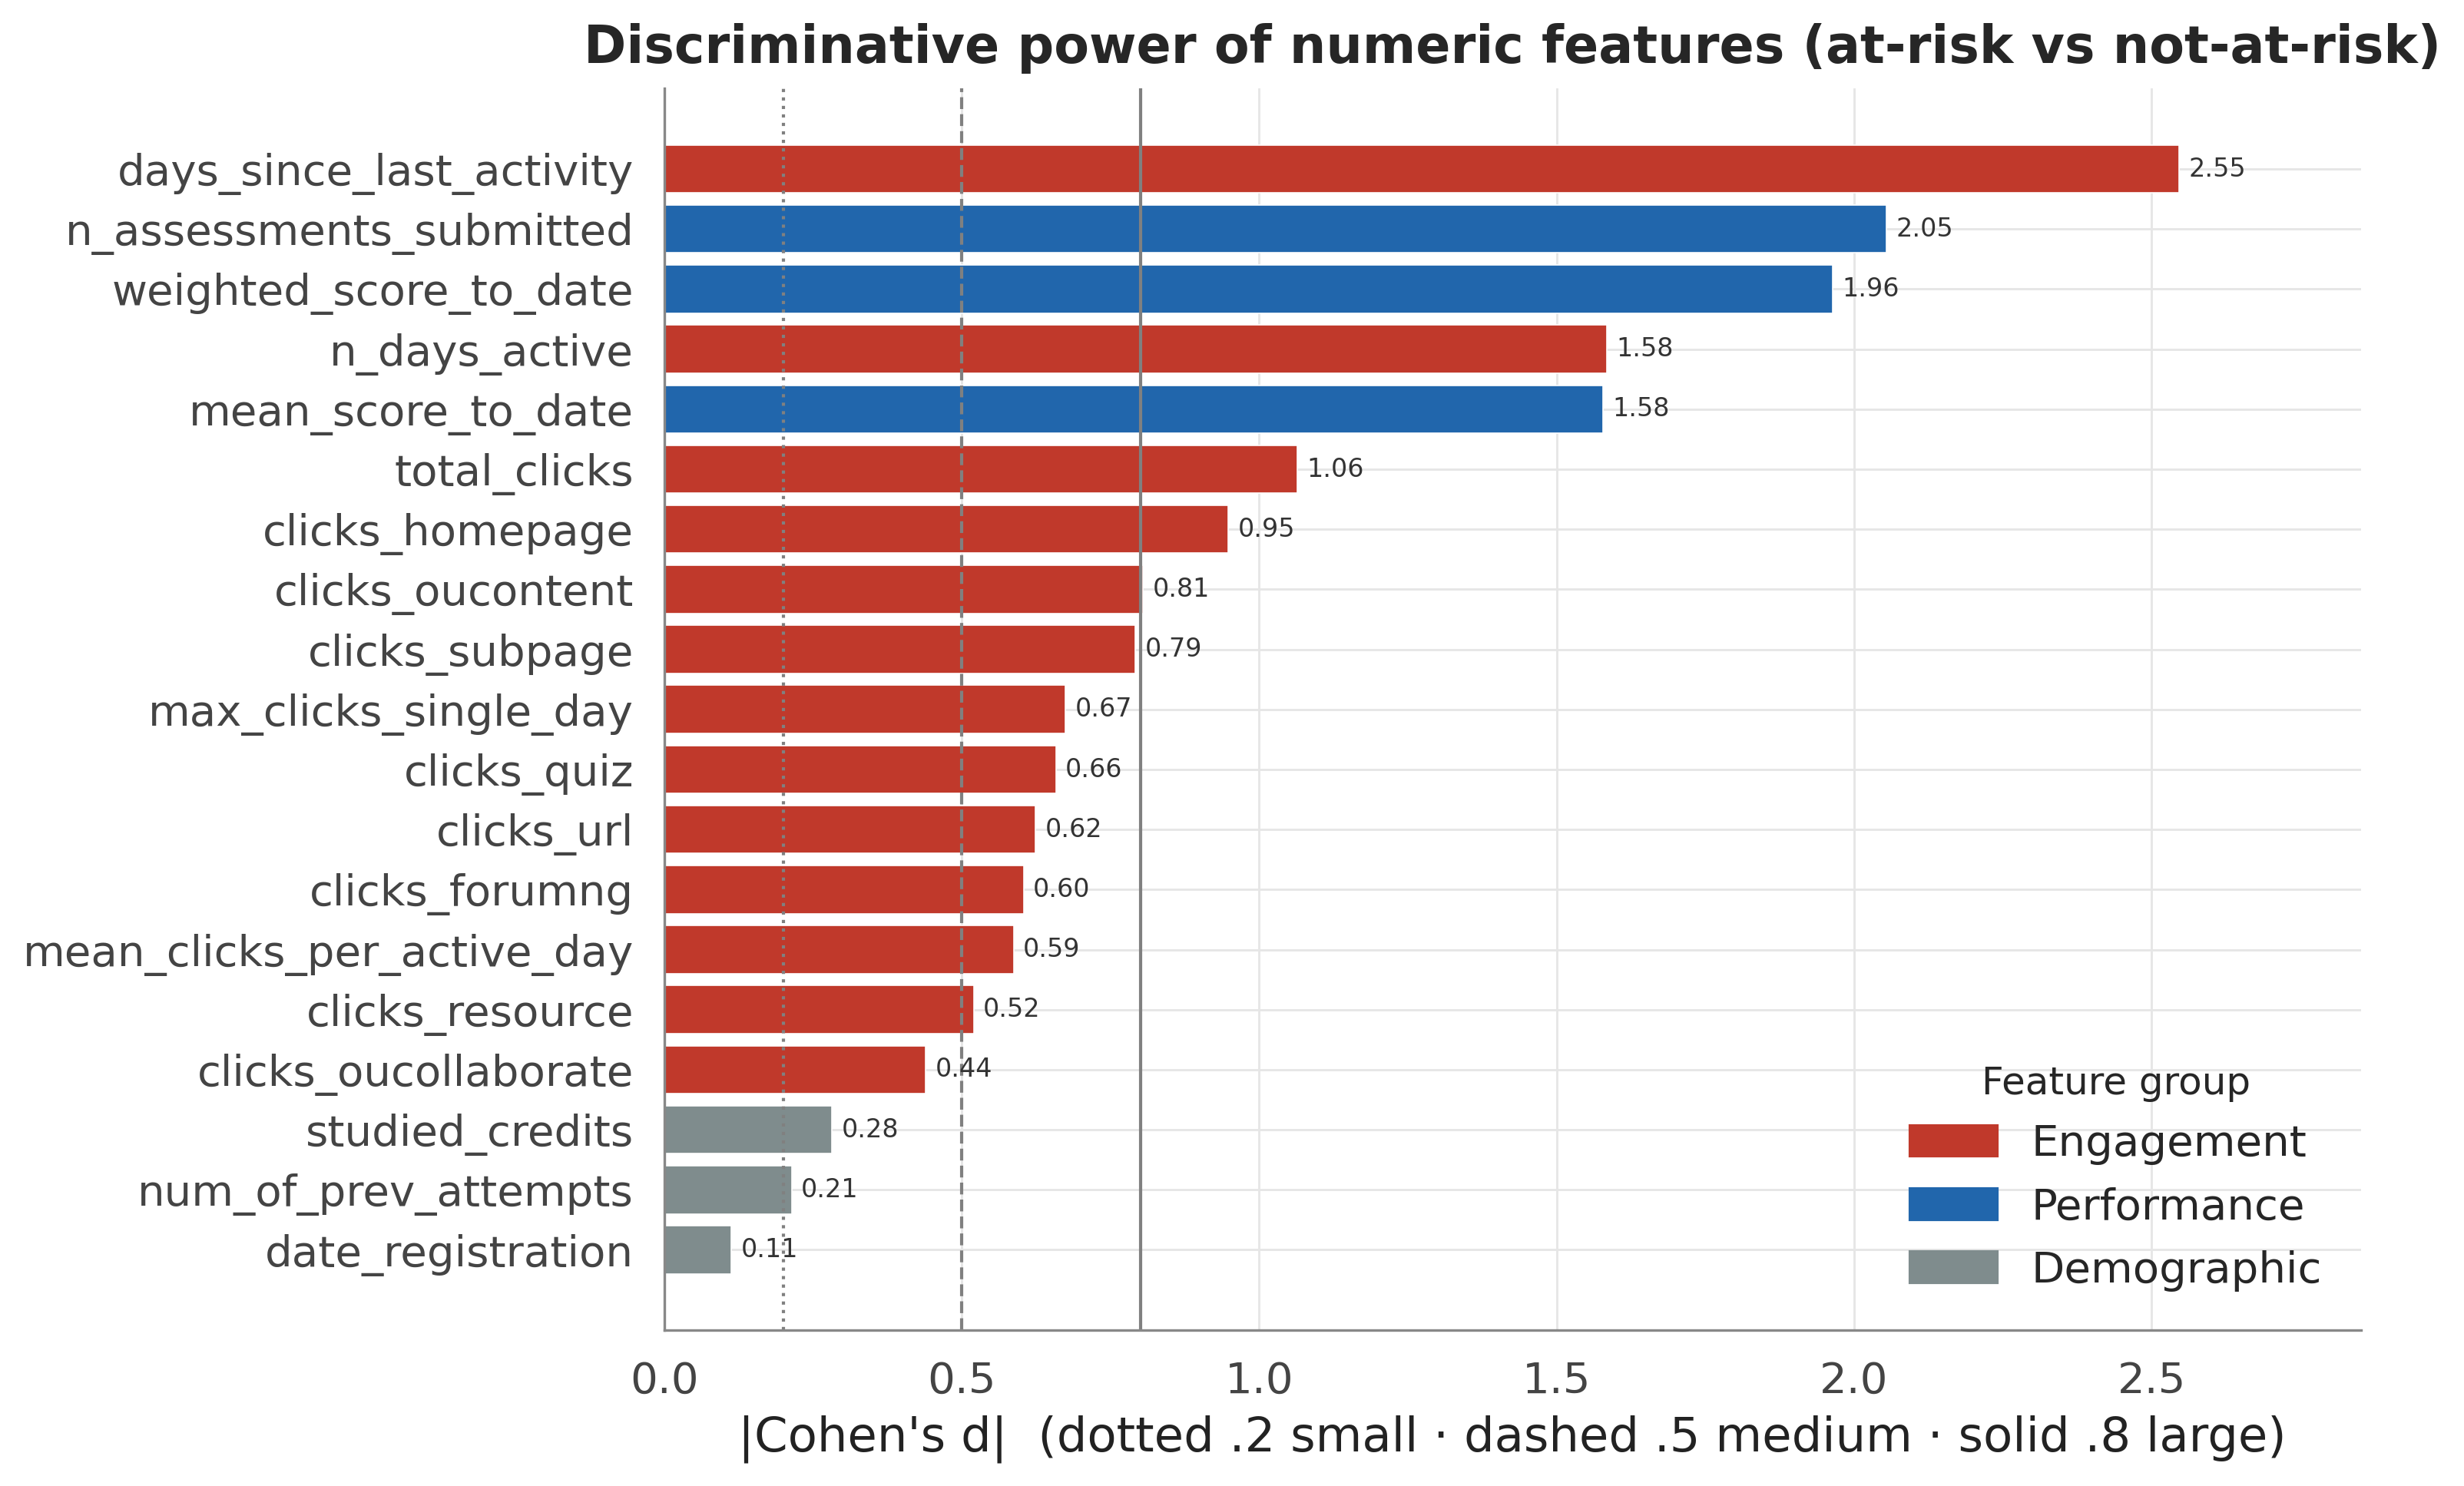
\includegraphics[width=\linewidth,height=0.74\textheight,keepaspectratio]{bivariate_effect_sizes.png}
    \end{column}
  \end{columns}
\end{frame}

\begin{frame}{Class Imbalance \& Plan}
  \wwr{Check: at-risk 52.8\% / not-at-risk 47.2\% $\to$ imbalance ratio 1.12 (mild).}
      {Missing an at-risk student is the costliest error $\to$ headline metrics are \textbf{PR-AUC \& recall} on the at-risk class.}
      {RQ3 plan: compare no-resampling / class-weight / SMOTE / ADASYN; resample on \textbf{train only}.}
\end{frame}

% ===================================================================== PART 5
\partframe{5}{Train/Test Split \& Leakage Control}{Văn Vinh}

\begin{frame}{Purpose, Ratio \& Split Method}
  \begin{itemize}\setlength\itemsep{0.4em}
    \item[\textcolor{cgreen}{\textbf{What}}]\, Ratio 80\% train / 20\% test (\code{TEST_SIZE = 0.2}).
    \item[\textcolor{cgreen}{\textbf{What}}]\, Method: \code{StratifiedGroupKFold} — stratify by \code{at_risk} + group by \code{id_student}.
    \item[\textcolor{cblue}{\textbf{Why}}]\, A student spans several module-presentations $\Rightarrow$ group by \code{id_student} so the same person is never in both train and test (group leakage).
    \item[\textcolor{themecol}{\textbf{Result}}]\, Test $\approx$ 6{,}489 rows / 5{,}756 students · train $\approx$ 26{,}104 rows.
  \end{itemize}
\end{frame}

\begin{frame}{Leakage Control — Two Axes}
  \begin{columns}[T]
    \begin{column}{0.5\textwidth}
      \wwr{Time axis: \code{cut_at_checkpoint()} keeps only events $\leq$ the checkpoint day; \code{cutoff = round(length × t/100)}. Feature axis: every learner (encoder, scaler, resampler) is \textbf{fit on train only}.}
          {Mirror exactly ``the information available at prediction time'' — no peeking into the future.}
          {6 datasets \code{dataset_t10}\ldots\code{t100}, identical student list; fixed at-risk 52.8\% across checkpoints.}
    \end{column}
    \begin{column}{0.5\textwidth}
      \centering
      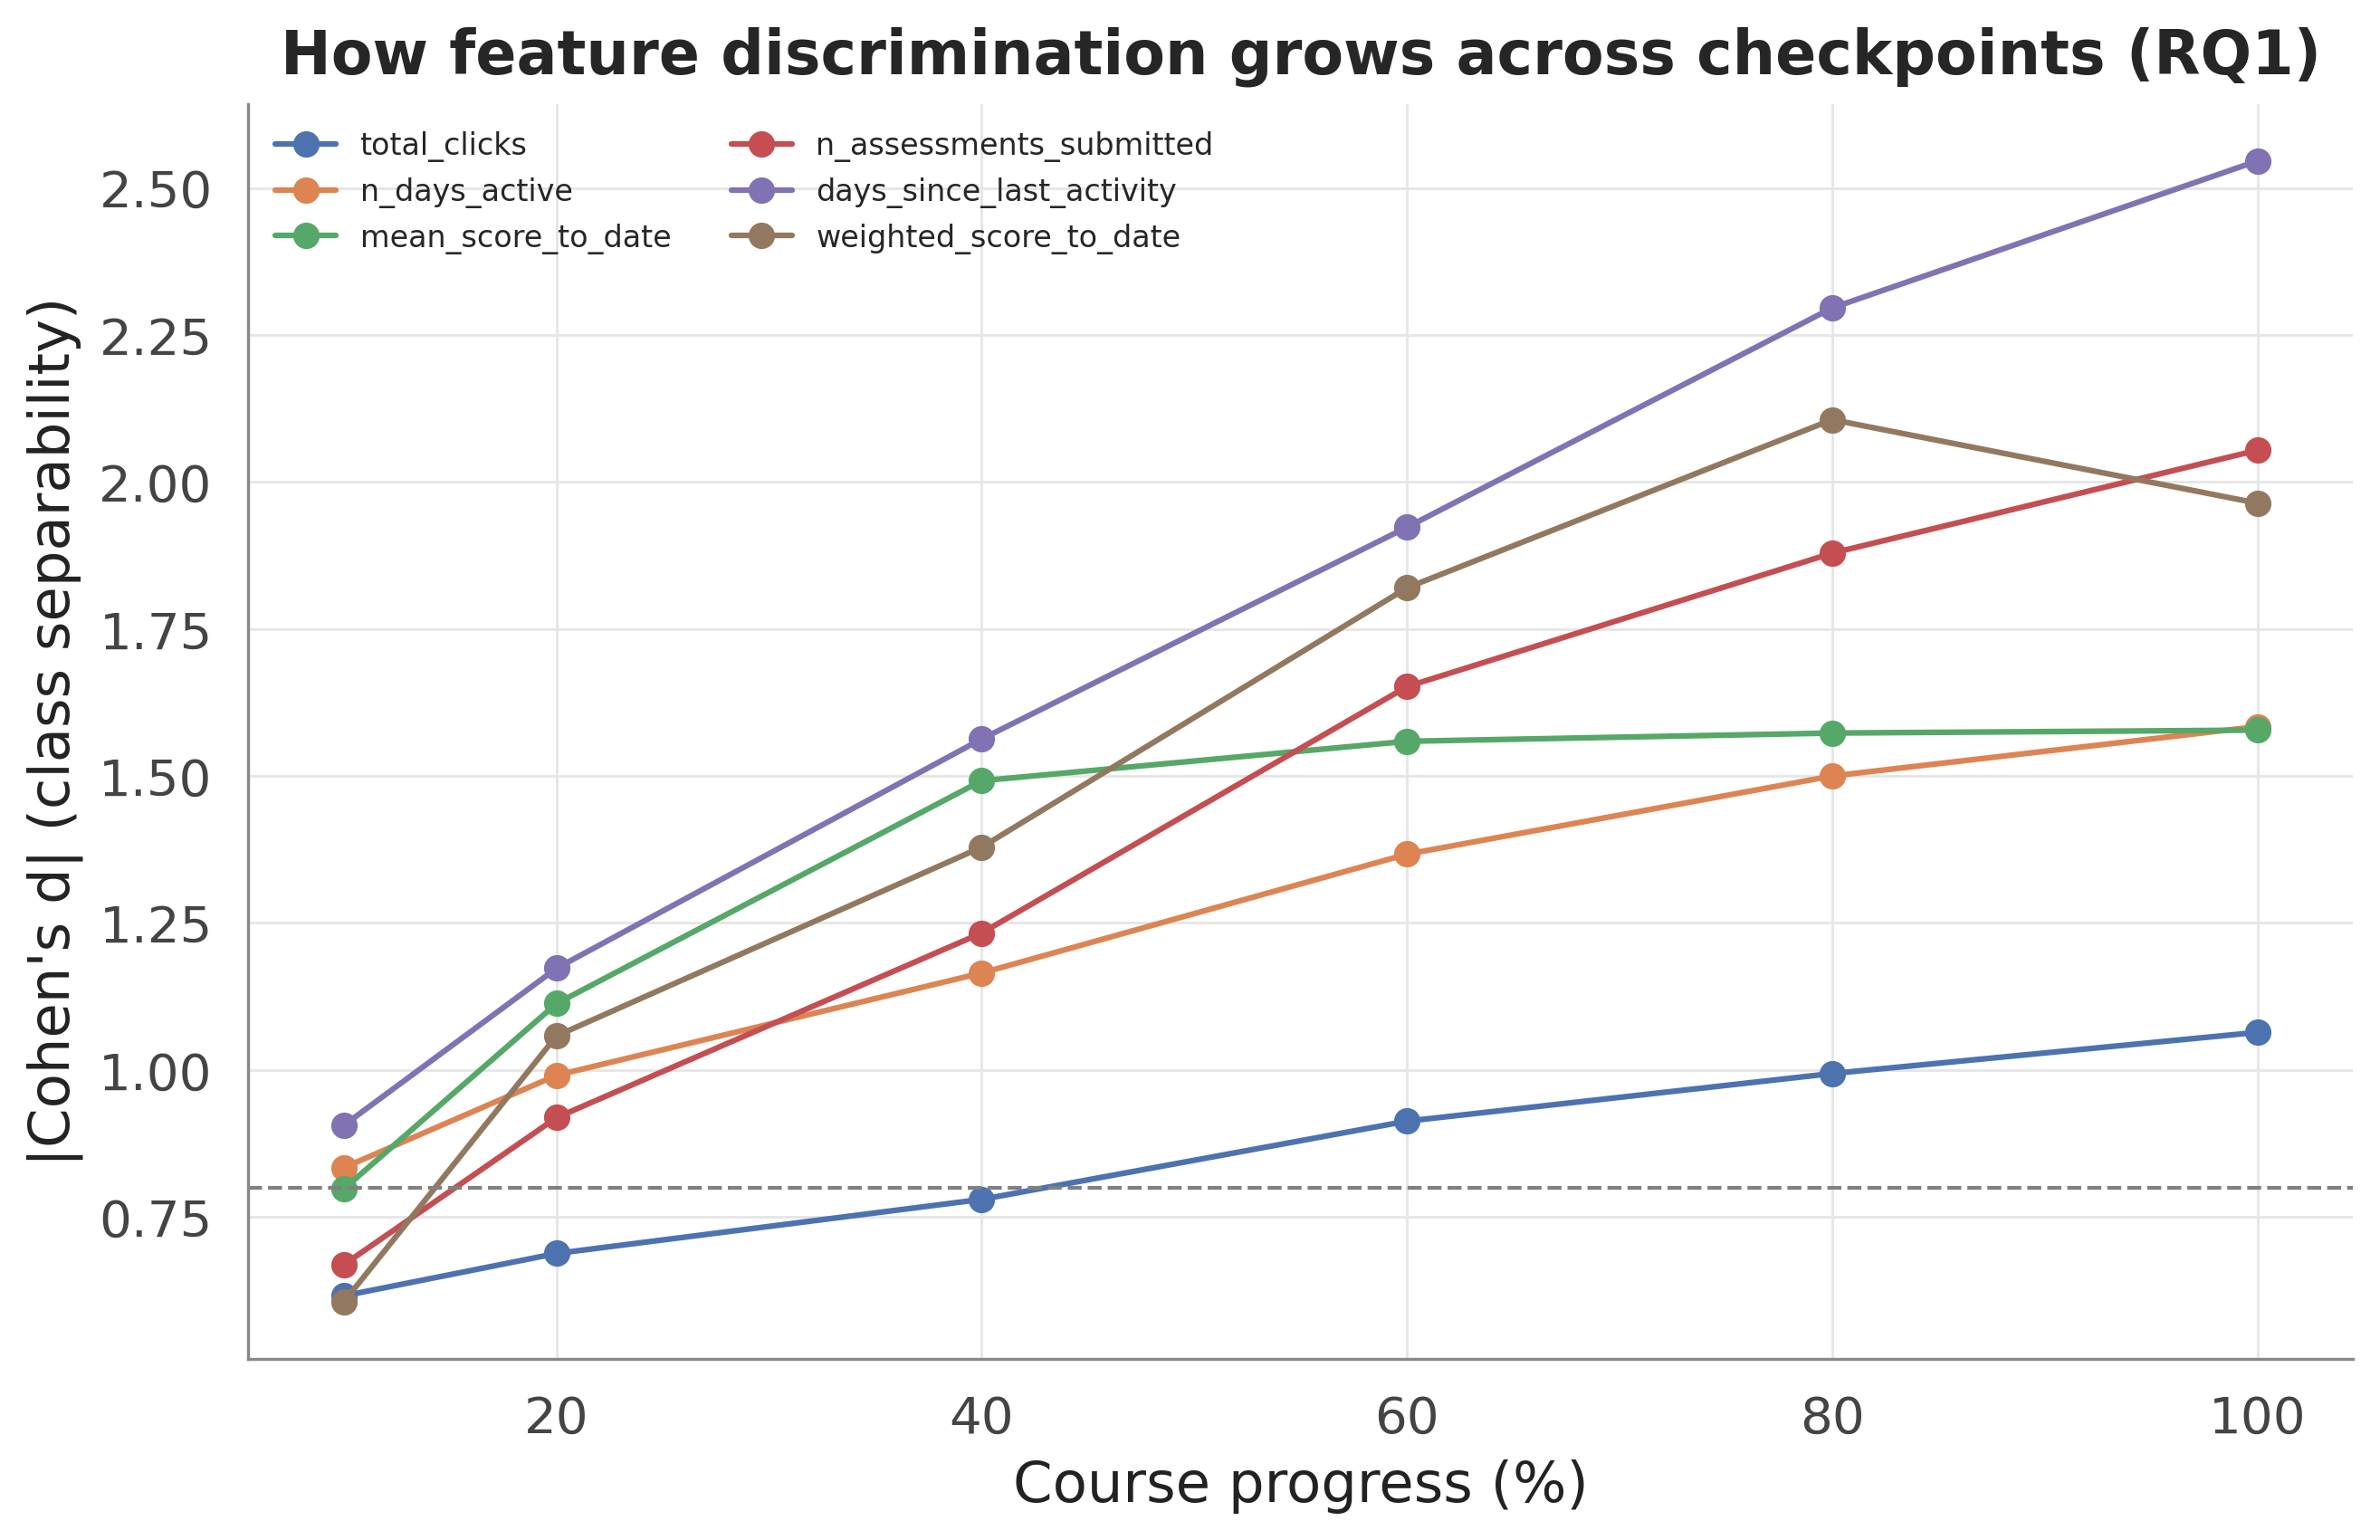
\includegraphics[width=\linewidth,height=0.7\textheight,keepaspectratio]{time_discrimination_curve.png}\\
      {\scriptsize\itshape Discrimination grows with time (RQ1)}
    \end{column}
  \end{columns}
\end{frame}

\begin{frame}{Correct Preprocessing Order (train$\to$test)}
  \wwr{Order: split train/test $\to$ impute $\to$ outliers $\to$ encode/scale $\to$ resample.}
      {Parameters (median, winsorise thresholds, mean/std, encoder categories) learned from train $\to$ applied to test. Fitting before the split leaks test into train $\Rightarrow$ fake results.}
      {Label distribution after split: train 0.53 / test 0.52 — gap $\leq$ 0.02, stratification holds.}
\end{frame}

\begin{frame}{Save \& Re-Verify — Leakage Blocked}
  \begin{itemize}\setlength\itemsep{0.4em}
    \item[\textcolor{cgreen}{\textbf{What}}]\, Save: \code{test_student_ids.csv} (committed) + train/test parquet; \code{split_report.csv}.
    \item[\textcolor{cgreen}{\textbf{What}}]\, Re-check: 0 students overlapping train/test; no type/column drift; balanced label.
    \item[\textcolor{cblue}{\textbf{Why}}]\, A fixed test, reused identically across all 6 checkpoints $\Rightarrow$ 6 \textbf{comparable} performance points.
  \end{itemize}
  \keynum{\code{tests/test_leakage.py}: \textbf{19/19} tests pass — automated evidence of no leakage.}
\end{frame}

% ===================================================================== Conclusion
\partframe{}{Conclusion}{}

\begin{frame}{Task 3 — Summary}
  {\footnotesize
  \setlength{\tabcolsep}{7pt}\renewcommand{\arraystretch}{1.35}
  \begin{tabularx}{\linewidth}{@{}>{\raggedright\arraybackslash}p{3.3cm} Y@{}}
    \toprule
    \rowcolor{themecol}\hc{Item} & \hc{Our result}\\
    \midrule
    1. Define data & binary \code{at_risk} 52.8\%; 3 groups; 32{,}593 student–module–presentation\\
    \rowcolor{rowtint}2. Collection & OULAD CC-BY 4.0; 7 tables; 10.6M clicks; MD5-verified\\
    3. Cleaning & 0 duplicates; log1p+winsorise, 0 rows dropped; master 32{,}593$\times$33\\
    \rowcolor{rowtint}4. Transform & Ordinal+OneHot+Binary; StandardScaler; d up to 2.55; RQ3 plan\\
    5. Train/test split & 80/20 group+stratified; 6 checkpoints; 19/19 tests pass\\
    \bottomrule
  \end{tabularx}}
  \takeaway{All five Task-3 items completed with concrete artifacts and figures.}
\end{frame}

\begin{frame}{Outputs \& Next Steps}
  \begin{itemize}\setlength\itemsep{0.5em}
    \item[\textcolor{themecol}{\textbf{Outputs}}]\, \code{master_raw} + 6 datasets \code{dataset_t10}\ldots\code{t100} + a fixed test set + a reproducible pipeline (seed=42, MD5, Restart \& Run All).
    \item[\textcolor{cgreen}{\textbf{Next}}]\, Benchmark models per checkpoint (RQ1) $\to$ handle imbalance (RQ3) $\to$ SHAP/LIME \& explanation stability (RQ2).
  \end{itemize}
  \vfill
  \begin{center}{\Large\color{themecol}\textbf{Thank you — questions welcome!}}\end{center}
  \vfill
\end{frame}

\end{document}
